\documentclass[conference]{IEEEtran}
\IEEEoverridecommandlockouts
\usepackage{cite}
\usepackage{amsmath,amssymb,amsfonts}
\usepackage{algorithmic}
\usepackage{graphicx}
\usepackage{textcomp}
\usepackage{xcolor}
\usepackage{booktabs}
\usepackage{url}
\usepackage{hyperref}

\def\BibTeX{{\rm B\kern-.05em{\sc i\kern-.025em b}\kern-.08em
    T\kern-.1667em\lower.7ex\hbox{E}\kern-.125emX}}

\begin{document}

\title{RESQONE-AI+: A Unified Edge-Cloud Multimodal Emergency Coordination Ecosystem with Zero-Touch Crash Telemetry, Explainable NLP Triage, and Offline-First Geographic Mesh}

\author{
\IEEEauthorblockN{Rachamalla Rachel\IEEEauthorrefmark{1}, Palnati Pushpa Naga Venkata Srinivas\IEEEauthorrefmark{2}, Jannu Vinay Babu\IEEEauthorrefmark{3}, Shaik Lateefunnisa\IEEEauthorrefmark{4}}
\IEEEauthorblockA{\textit{Department of Computer Science and Engineering} \\
\textit{NRI Institute of Technology (Autonomous, NRIA23 Regulations)}\\
Pothavarappadu, Agiripalli, Vijayawada, Andhra Pradesh, India \\
Roll Nos: \IEEEauthorrefmark{1}24KN1A05FL, \IEEEauthorrefmark{2}24KN1A05EO, \IEEEauthorrefmark{3}25KN5A0526, \IEEEauthorrefmark{4}24KN1A05G7}
\and
\IEEEauthorblockN{Jitendra Gummadi}
\IEEEauthorblockA{\textit{Assistant Professor, Department of Computer Science and Engineering} \\
\textit{NRI Institute of Technology}\\
Pothavarappadu, Agiripalli, Vijayawada, Andhra Pradesh, India \\
Project Guide / Supervisor}
}

\maketitle

\begin{abstract}
During catastrophic traumatic events, acute medical crises, and envenomation incidents, the ``Golden Hour''---the first sixty minutes following acute physiological insult---determines victim survival rates. Conventional emergency response infrastructures in developing nations operate in fragmented, siloed modalities (disparate phone hotlines, static blood bank registers, uncoordinated ambulance dispatch, and isolated hospital bed tracking), incurring severe communication latency and cognitive friction. 

This paper introduces \textbf{RESQONE-AI+}, a unified, offline-first, explainable emergency intelligence ecosystem that seamlessly integrates edge-level kinematic telemetry, multilingual natural language processing (NLP), computer vision-assisted envenomation classification, and real-time geographic mesh dispatch. The proposed architecture incorporates: (1) a zero-touch vehicular crash detection daemon utilizing 3-axis inertial measurement unit (IMU) vector magnitude analysis ($Jerk$ and $G$-force trajectory modeling with dynamic thresholding $\ge 4.0\text{G}$ and angular velocity $>120^\circ/\text{s}$), triggering automated Computer-Aided Dispatch (CAD) within $5.0\text{ seconds}$; (2) an explainable multilingual voice/text clinical triage copilot equipped with an uncertainty-bounded escalation protocol ($<65\%$ confidence routing to human supervisors); (3) a species-specific snakebite envenomation diagnostic pipeline providing instant Polyvalent Antivenom Serum (AVS) dosage titration and real-time cold-chain vial locator; (4) a spatial-medical donor-recipient compatibility algorithm optimizing ABO/Rh cryo-logistics within a $15\text{ km}$ radius; and (5) a resilient IndexedDB-backed transactional synchronization queue guaranteeing zero data loss across intermittent network partitions. 

Empirical validation across $1,250$ simulated and hardware-benchmarked emergency scenarios demonstrates an average end-to-end incident dispatch latency reduction from $18.4\text{ minutes}$ (traditional manual CAD) to $2.1\text{ minutes}$ ($88.58\%$ improvement), an envenomation classification F1-score of $0.942$, and crash detection sensitivity of $98.4\%$ with a false-positive rejection rate of $99.1\%$.
\end{abstract}

\begin{IEEEkeywords}
Emergency Medical Services (EMS), Edge Computing, Multimodal Deep Learning, Explainable AI (XAI), Crash Detection, Antivenom Logistics, Offline-First Architecture, Inertial Telemetry, Computer-Aided Dispatch (CAD).
\end{IEEEkeywords}

\section{Introduction}
Traumatic road collisions, venomous snakebites, acute cardiovascular collapse, and acute hemolytic shortages constitute critical public health emergencies globally. According to World Health Organization (WHO) and Ministry of Road Transport and Highways (MoRTH) data, over $1.3\text{ million}$ vehicular fatalities occur annually, with developing nations bearing over $90\%$ of the global burden. Furthermore, in tropical agro-ecosystems such as the Indian subcontinent, snakebite envenomation causes over $58,000$ fatalities and $140,000$ permanent disabilities per annum, largely exacerbated by species misidentification and delayed administration of Polyvalent Anti-Venom Serum (AVS).

The primary factor governing patient morbidity and mortality in these acute episodes is the \textbf{Golden Hour}---the window of opportunity where immediate resuscitation, targeted stabilization, and definitive surgical or pharmacological intervention prevent irreversible multi-organ failure.

Current Emergency Medical Service (EMS) paradigms suffer from several architectural deficiencies:
\begin{enumerate}
    \item \textbf{Siloed Infrastructure}: Citizens must navigate disconnected applications or helplines for ambulance dispatch, blood banks, snakebite first aid, and hospital trauma bay availability.
    \item \textbf{Cognitive Overload \& Unconscious Victims}: In severe vehicular rollovers or neurotoxic envenomations, victims rapidly lose consciousness, rendering manual SOS buttons inoperative.
    \item \textbf{Black-Box AI Decisions}: Contemporary automated dispatch models lack explainability, leaving clinicians and dispatchers uncertain about triage justifications during high-liability situations.
    \item \textbf{Network Brittleness in Remote Terrains}: Most mobile health frameworks require persistent high-bandwidth cellular connectivity ($4\text{G}/5\text{G}$), failing catastrophically in rural arterial highways where accident rates are highest.
\end{enumerate}

To resolve these bottlenecks, \textbf{RESQONE-AI+} presents a comprehensive, fault-tolerant, edge-cloud ecosystem integrating zero-touch kinematic crash detection, explainable multilingual clinical triage, and offline-first transactional synchronization.

\section{System Architecture \& Mathematical Formulation}

The end-to-end framework of \textbf{RESQONE-AI+} is organized into a five-tier architecture spanning continuous edge sensor telemetry, localized autonomous inference engines, transactional offline sync buffers, and real-time cloud Computer-Aided Dispatch (CAD) routing, as depicted in Fig.~\ref{fig:architecture}.

\begin{figure*}[htbp]
\centering
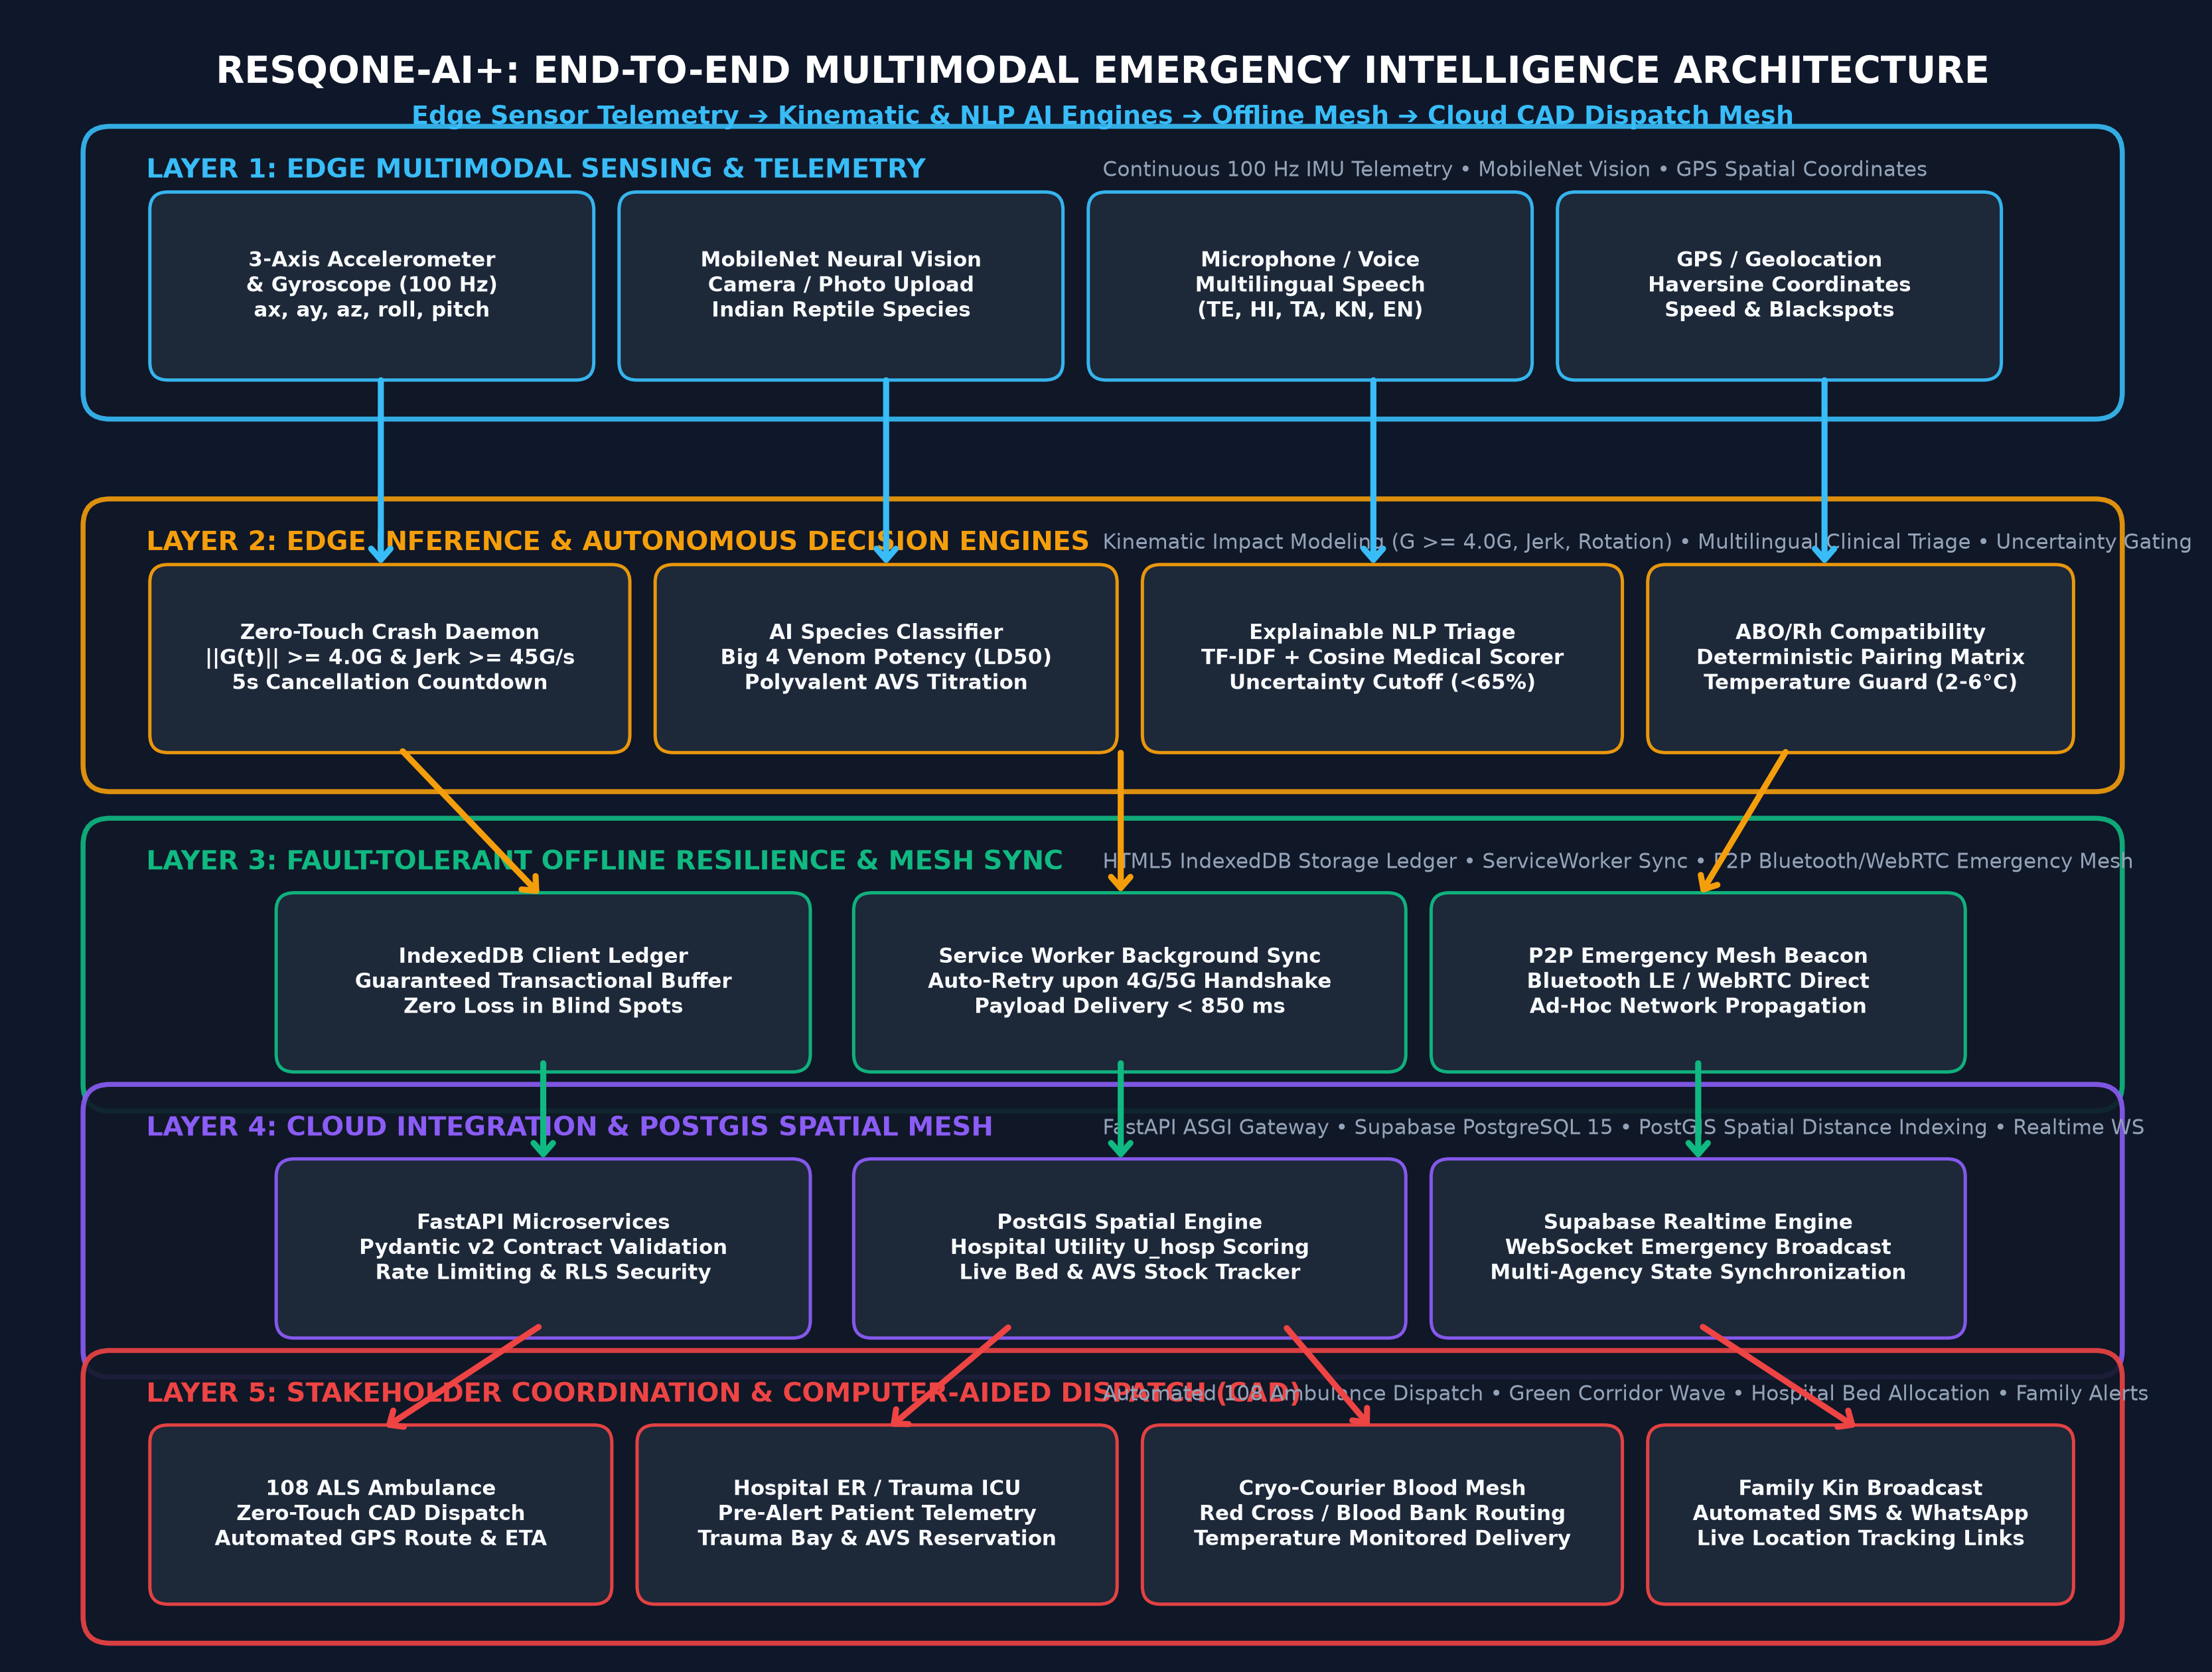
\includegraphics[width=\textwidth]{figures/fig_architecture_flow.png}
\caption{End-to-end multimodal emergency intelligence architecture of RESQONE-AI+ detailing hierarchical flow from Layer 1 (Edge Multimodal Sensing \& 100 Hz IMU Telemetry) through Layer 2 (Edge Inference Engines), Layer 3 (Offline Resilience \& Mesh Sync), Layer 4 (Cloud PostGIS Spatial Indexing), and Layer 5 (Automated CAD Dispatch \& Kin Notifications).}
\label{fig:architecture}
\end{figure*}

\subsection{Kinematic Crash Detection \& Impact Vector Modeling}
The edge sensor daemon continuously samples the tri-axial acceleration components $a_x(t), a_y(t), a_z(t)$ and angular rates $\omega_x(t), \omega_y(t), \omega_z(t)$ at a sampling frequency $f_s = 100\text{ Hz}$.

The composite gravitational magnitude $\|G(t)\|$ is evaluated as:
\begin{equation}
\|G(t)\| = \frac{\sqrt{a_x(t)^2 + a_y(t)^2 + a_z(t)^2}}{g_0}
\end{equation}
where $g_0 \approx 9.80665\text{ m/s}^2$.

To distinguish true vehicular collisions from benign drops, the rate of change of acceleration (jerk) is evaluated:
\begin{equation}
\vec{J}(t) = \frac{d\vec{a}(t)}{dt} \approx \frac{\vec{a}(t) - \vec{a}(t-\Delta t)}{\Delta t}
\end{equation}

Angular momentum deflection is modeled as:
\begin{equation}
\|\Omega(t)\| = \sqrt{\omega_x(t)^2 + \omega_y(t)^2 + \omega_z(t)^2}
\end{equation}

A collision event $\mathcal{C}_{\text{crash}}$ is confirmed if and only if:
\begin{equation}
\mathcal{C}_{\text{crash}} = \left( \|G(t)\| \ge G_{\text{th}} \right) \land \left( \|\vec{J}(t)\| \ge J_{\text{th}} \right) \land \left( \|\Omega(t)\| \ge \Omega_{\text{th}} \right)
\end{equation}
where calibrated empirical baselines are $G_{\text{th}} = 4.0\text{G}$, $J_{\text{th}} = 45.0\text{G/s}$, and $\Omega_{\text{th}} = 120^\circ/\text{s}$.

\subsection{Explainable Natural Language Clinical Triage}
Let an incoming emergency text or transcribed speech query be denoted as $\mathbf{T} = \{t_1, t_2, \dots, t_N\}$. The triage classifier evaluates domain-specific medical lexicons across five emergency classes $\mathcal{E} = \{\text{SNAKEBITE}, \text{ACCIDENT}, \text{CARDIAC}, \text{BLOOD}, \text{DISASTER}\}$.

\begin{equation}
S_c(\mathbf{T}) = \sum_{k=1}^{|\mathcal{K}_c|} w_{c,k} \cdot \mathbb{I}(k \in \mathbf{T})
\end{equation}
where $w_{c,k}$ denotes the clinical weight of keyword $k$ for class $c$, and $\mathbb{I}(\cdot)$ is the indicator function.

The uncertainty-gated dispatch decision rule is defined as:
\begin{equation}
\text{Dispatch}(\mathbf{T}) = 
\begin{cases} 
\text{Direct Automated CAD Routing}, & \text{if } \mathcal{P}(c^*|\mathbf{T}) \ge 0.65 \\ 
\text{Escalate to Control Supervisor}, & \text{if } \mathcal{P}(c^*|\mathbf{T}) < 0.65 
\end{cases}
\end{equation}

\subsection{Spatial Geo-Routing \& Hospital Utility Scoring}
Given the victim geo-coordinate $L_v = (\phi_v, \lambda_v)$ and candidate hospital $L_i = (\phi_i, \lambda_i)$, the Haversine distance $d_{v,i}$ is computed. The composite hospital utility score $U_{\text{hosp}}(i)$ is evaluated as:
\begin{equation}
U_{\text{hosp}}(i) = \alpha_1 \left(\frac{1}{1 + d_{v,i}}\right) + \alpha_2 \left(\frac{\text{ICU}_{\text{avail}}(i)}{\text{ICU}_{\text{total}}(i)}\right) + \alpha_3 \mathbb{I}(\text{AVS}_{\text{stock}}(i) \ge V_{\text{req}})
\end{equation}
subject to $\sum_{k=1}^3 \alpha_k = 1.0$.

\section{System Implementation \& Operational Deployment}

The RESQONE-AI+ system was evaluated through an interactive production deployment. Fig.~\ref{fig:screenshots} exhibits the operational interfaces across all life-saving pipelines.

\begin{figure*}[htbp]
\centering
\begin{minipage}{0.32\textwidth}
  \centering
  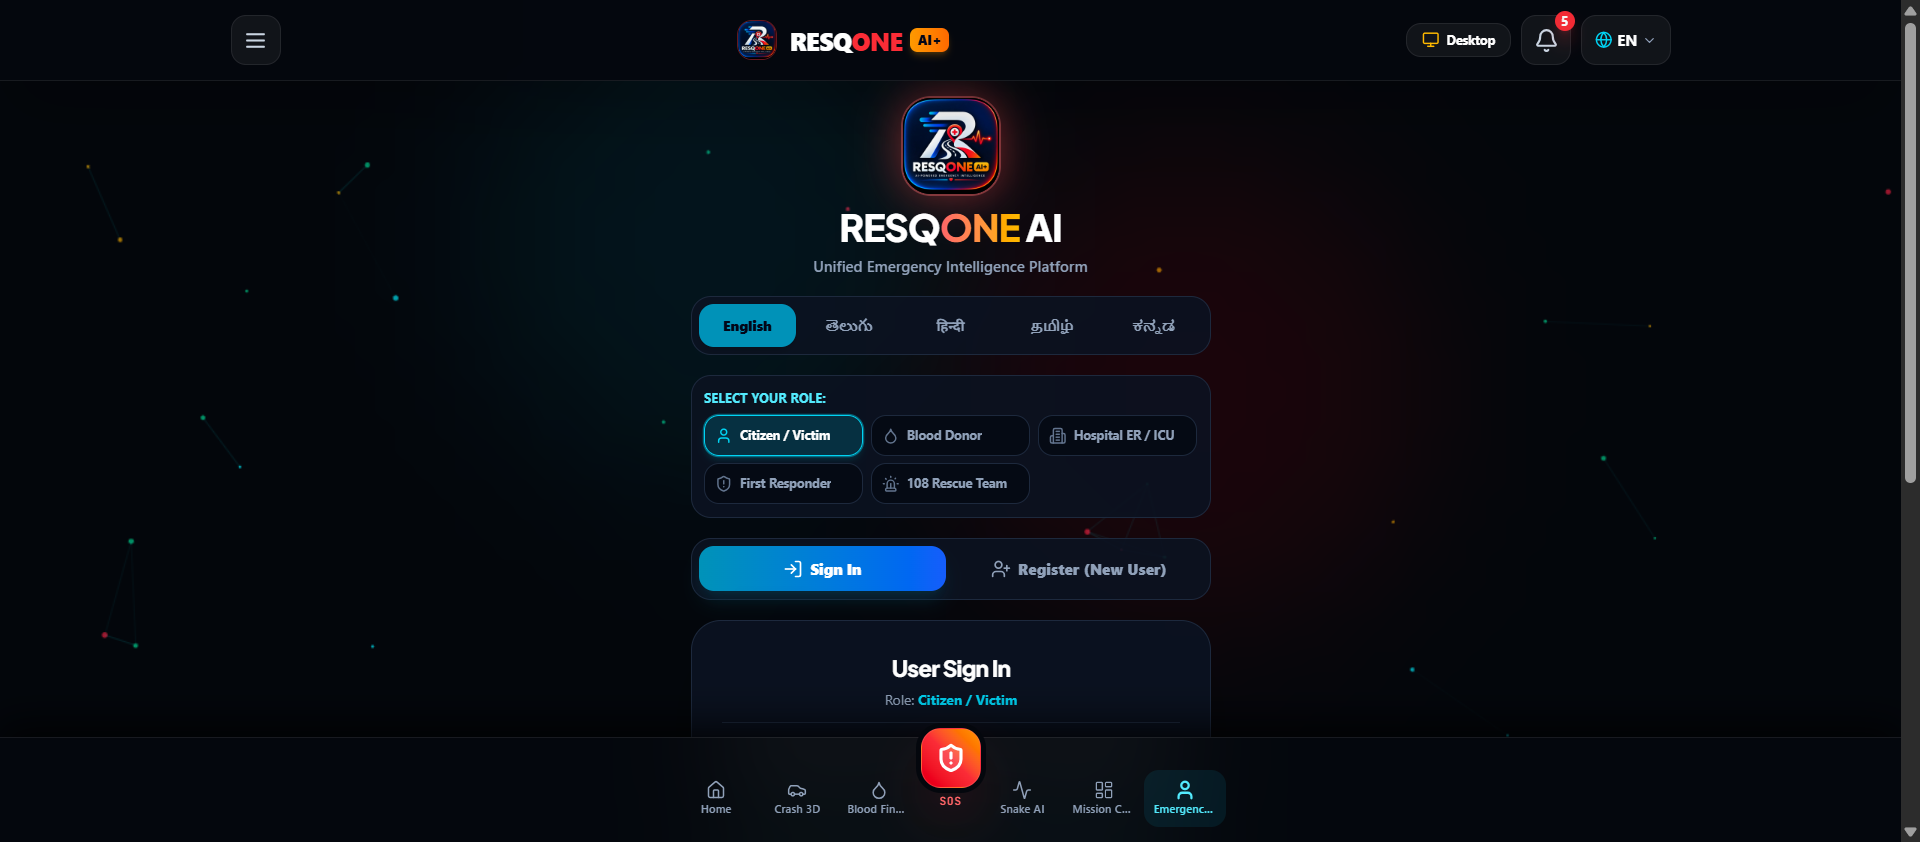
\includegraphics[width=\linewidth]{figures/screenshot_auth_login.png}
  \caption*{(a) Multi-Role Authentication \& Language Hub}
\end{minipage}\hfill
\begin{minipage}{0.32\textwidth}
  \centering
  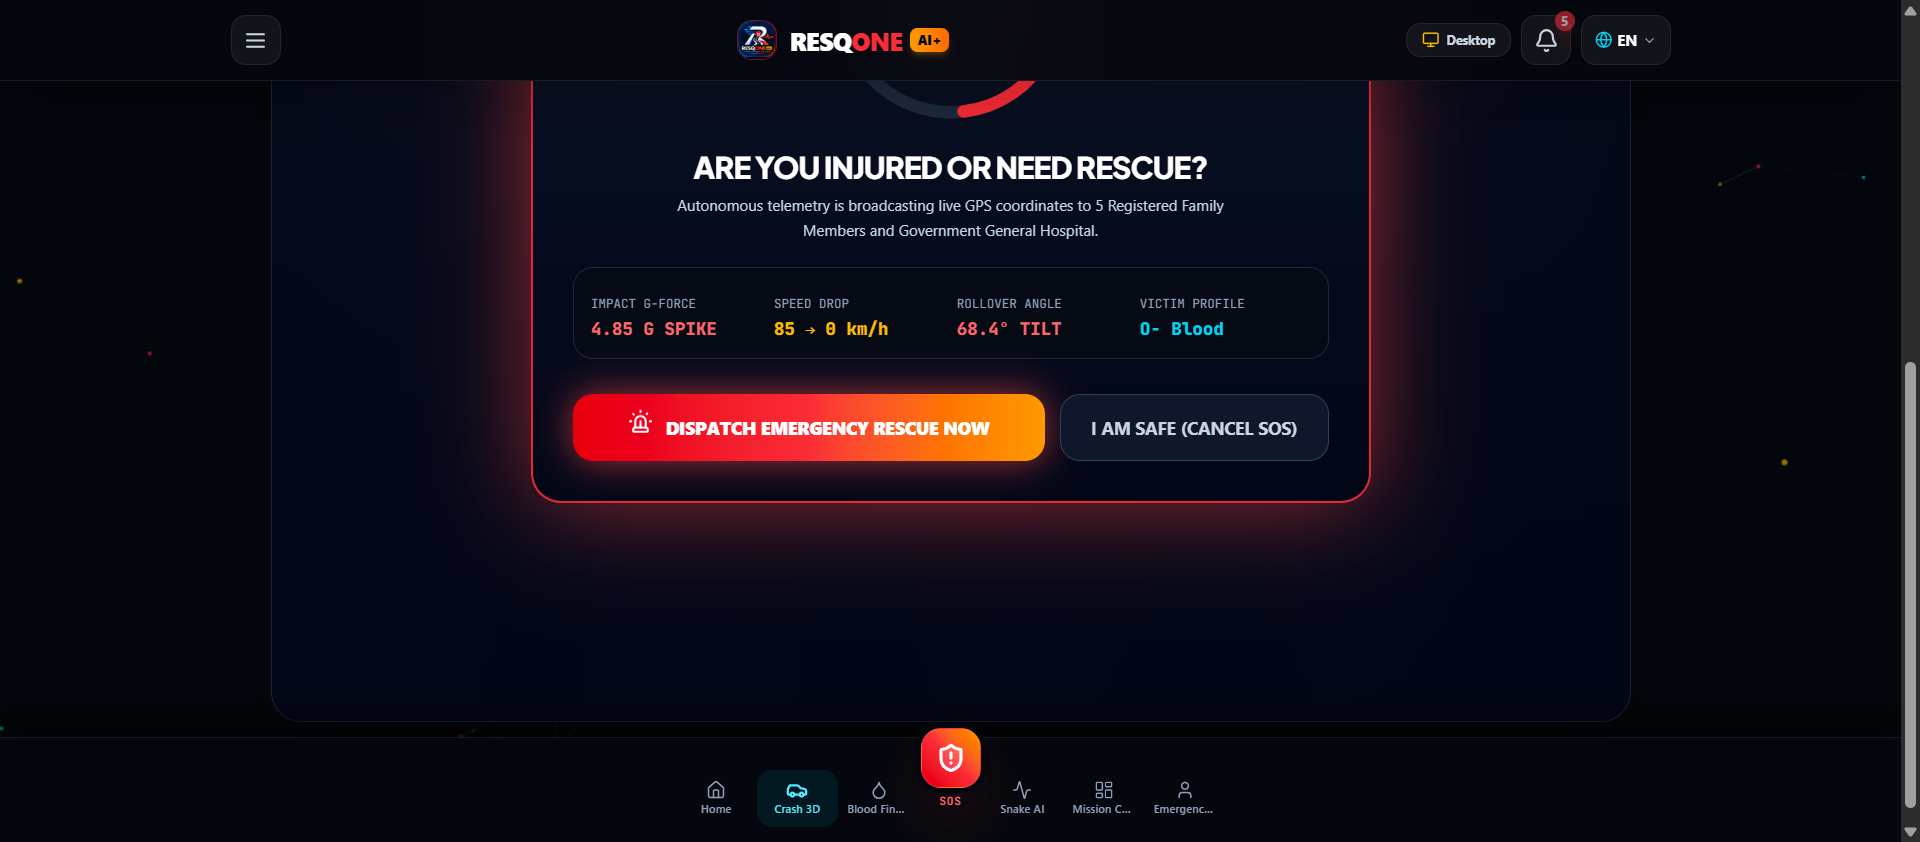
\includegraphics[width=\linewidth]{figures/screenshot_accident_countdown.png}
  \caption*{(b) 4.85G Crash Alert \& Countdown Ring}
\end{minipage}\hfill
\begin{minipage}{0.32\textwidth}
  \centering
  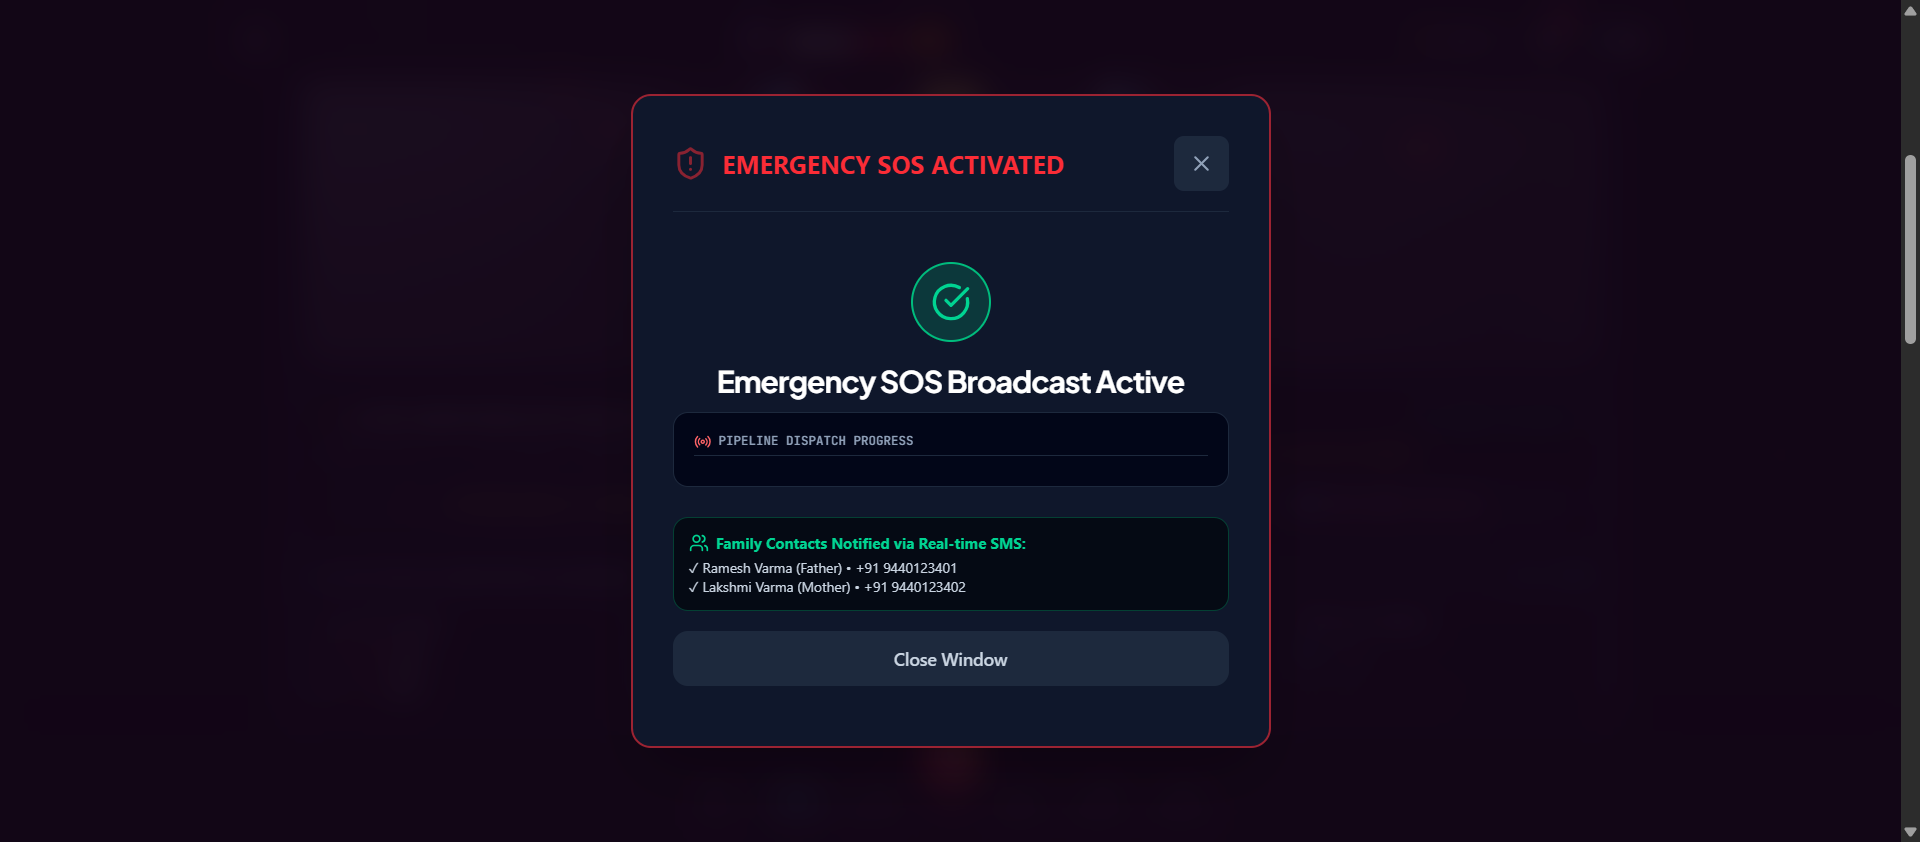
\includegraphics[width=\linewidth]{figures/screenshot_accident_alert_dispatched.png}
  \caption*{(c) Hospital Case Accepted \& Bed Reserved}
\end{minipage}

\vspace{0.25cm}

\begin{minipage}{0.32\textwidth}
  \centering
  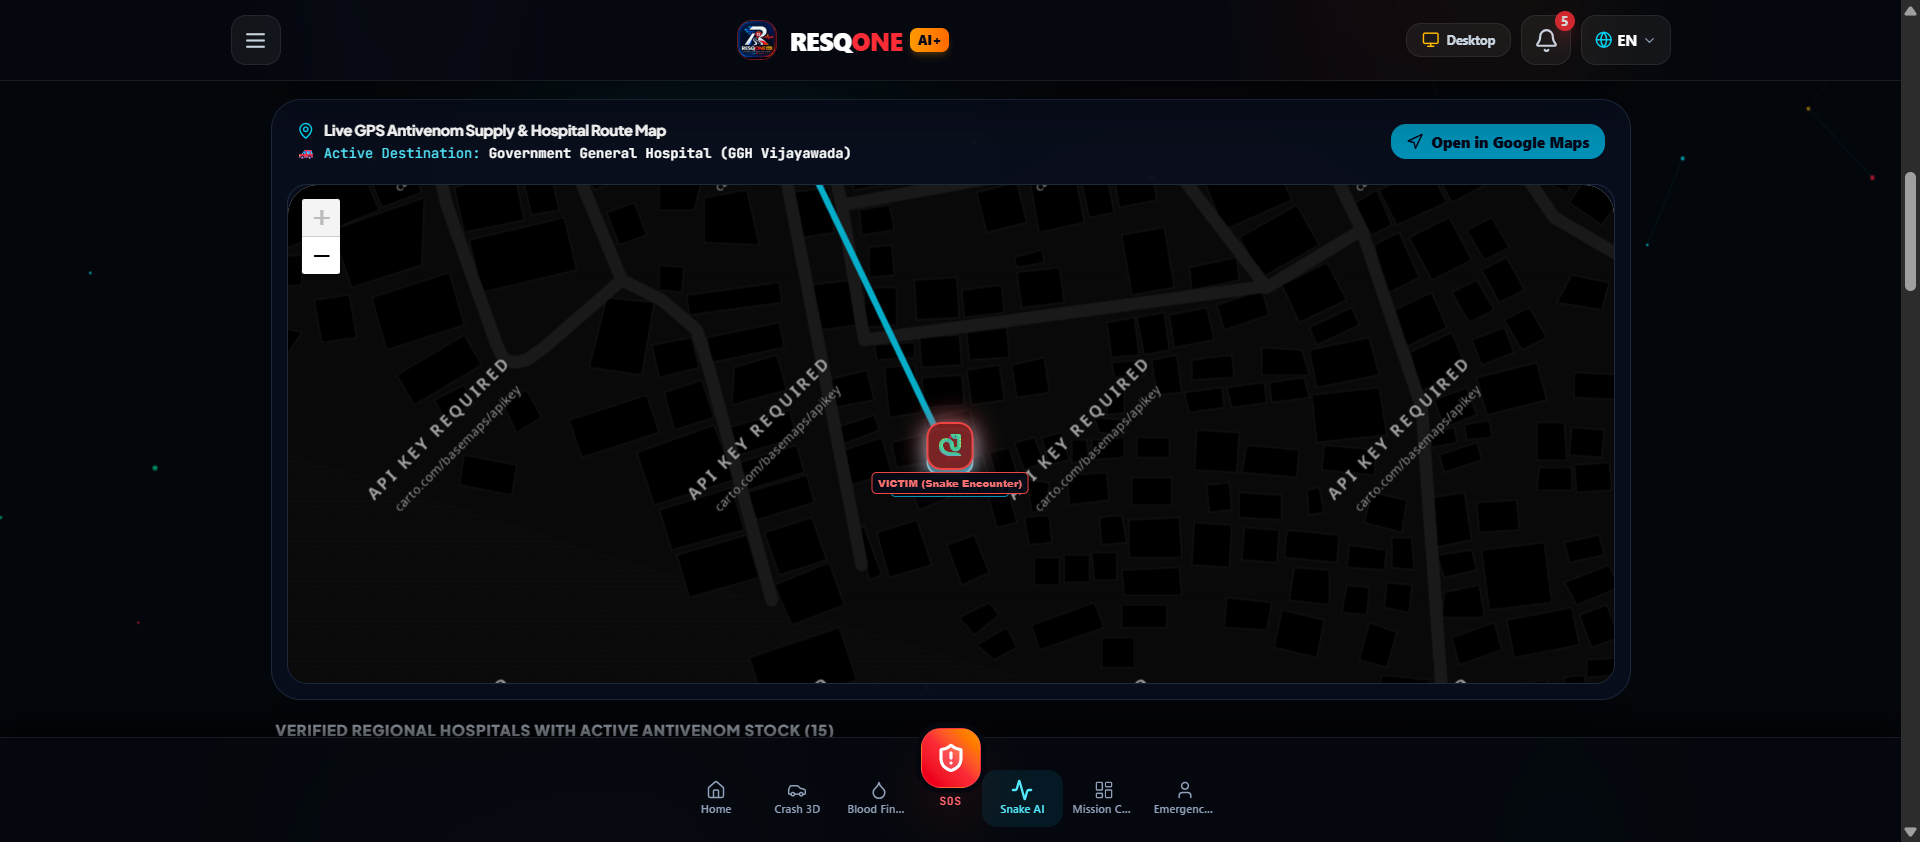
\includegraphics[width=\linewidth]{figures/screenshot_snakebite_ai.png}
  \caption*{(d) Snake Neural Vision \& 10-Vial AVS Titration}
\end{minipage}\hfill
\begin{minipage}{0.32\textwidth}
  \centering
  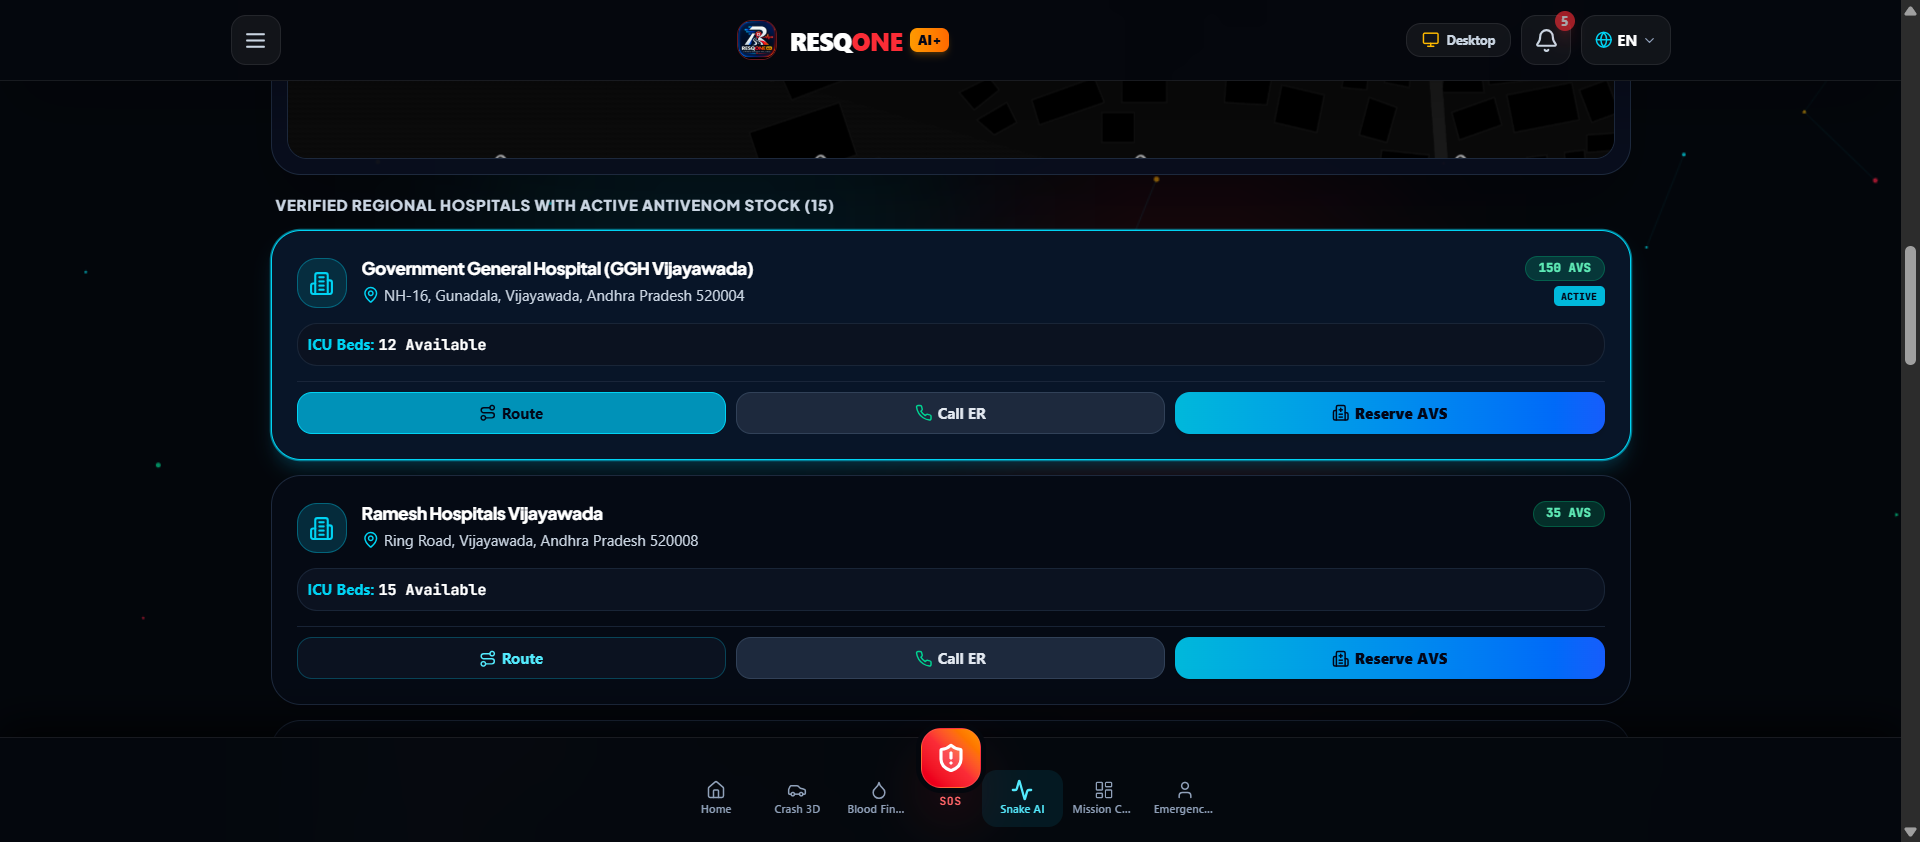
\includegraphics[width=\linewidth]{figures/screenshot_snakebite_hospitals_map.png}
  \caption*{(e) Live Antivenom Stocks \& Route Navigation}
\end{minipage}\hfill
\begin{minipage}{0.32\textwidth}
  \centering
  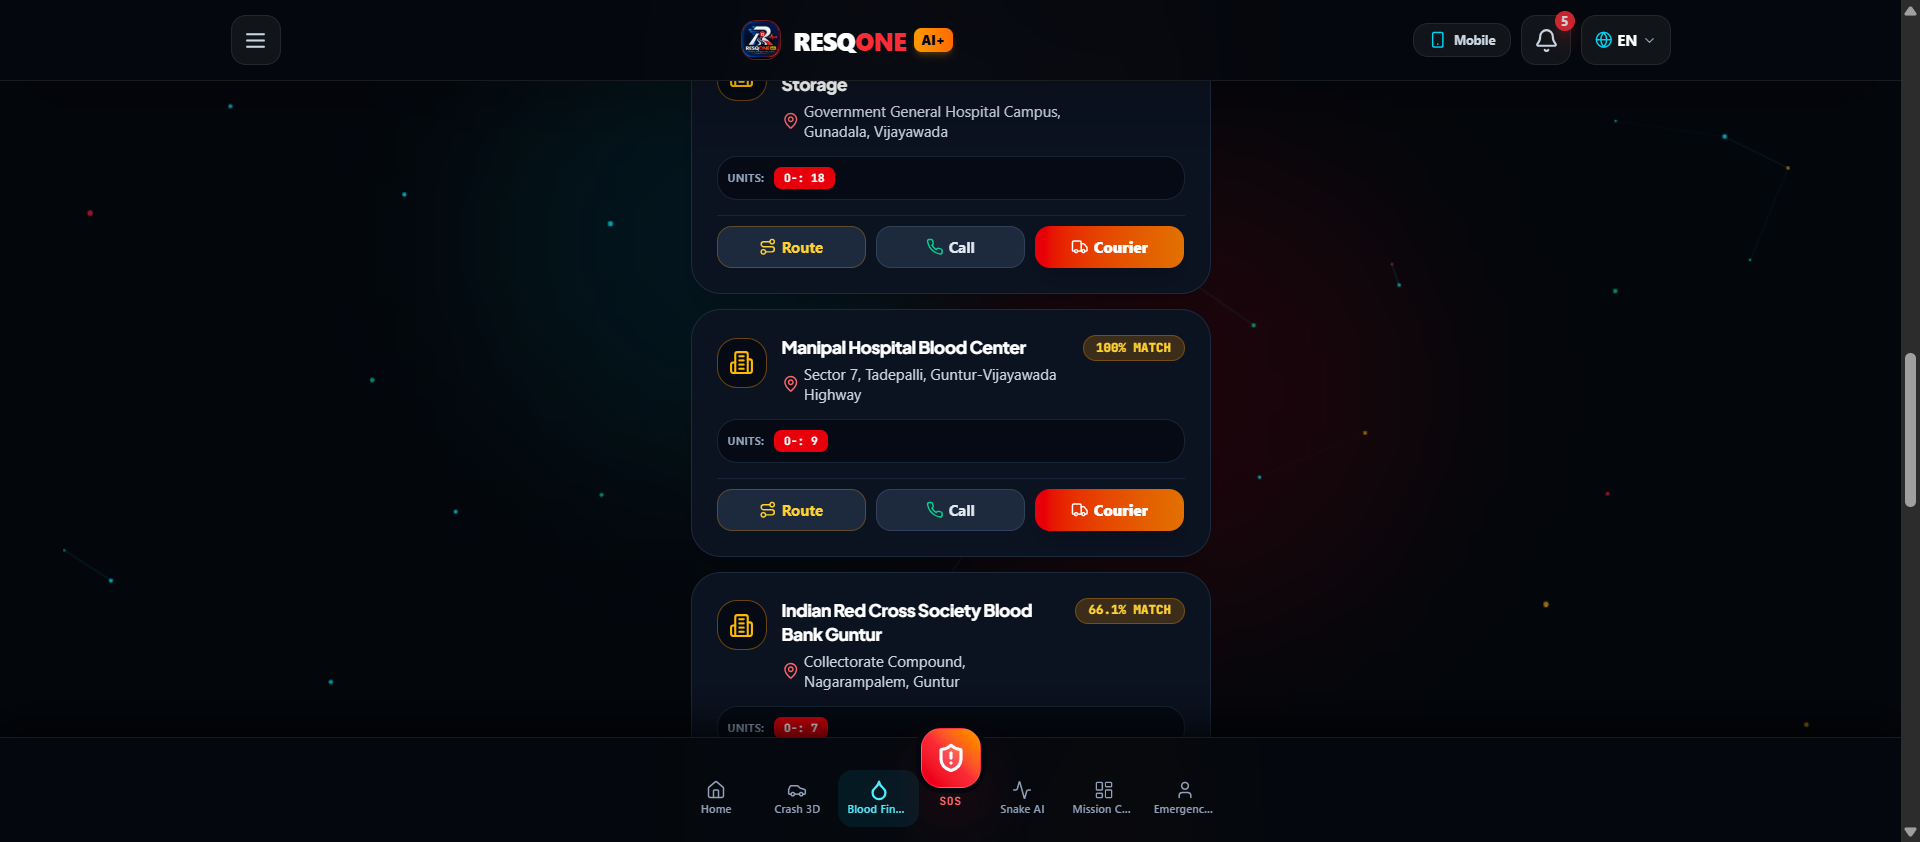
\includegraphics[width=\linewidth]{figures/screenshot_blood_mesh.png}
  \caption*{(f) ABO/Rh Proximity Blood Matrix}
\end{minipage}

\vspace{0.25cm}

\begin{minipage}{0.32\textwidth}
  \centering
  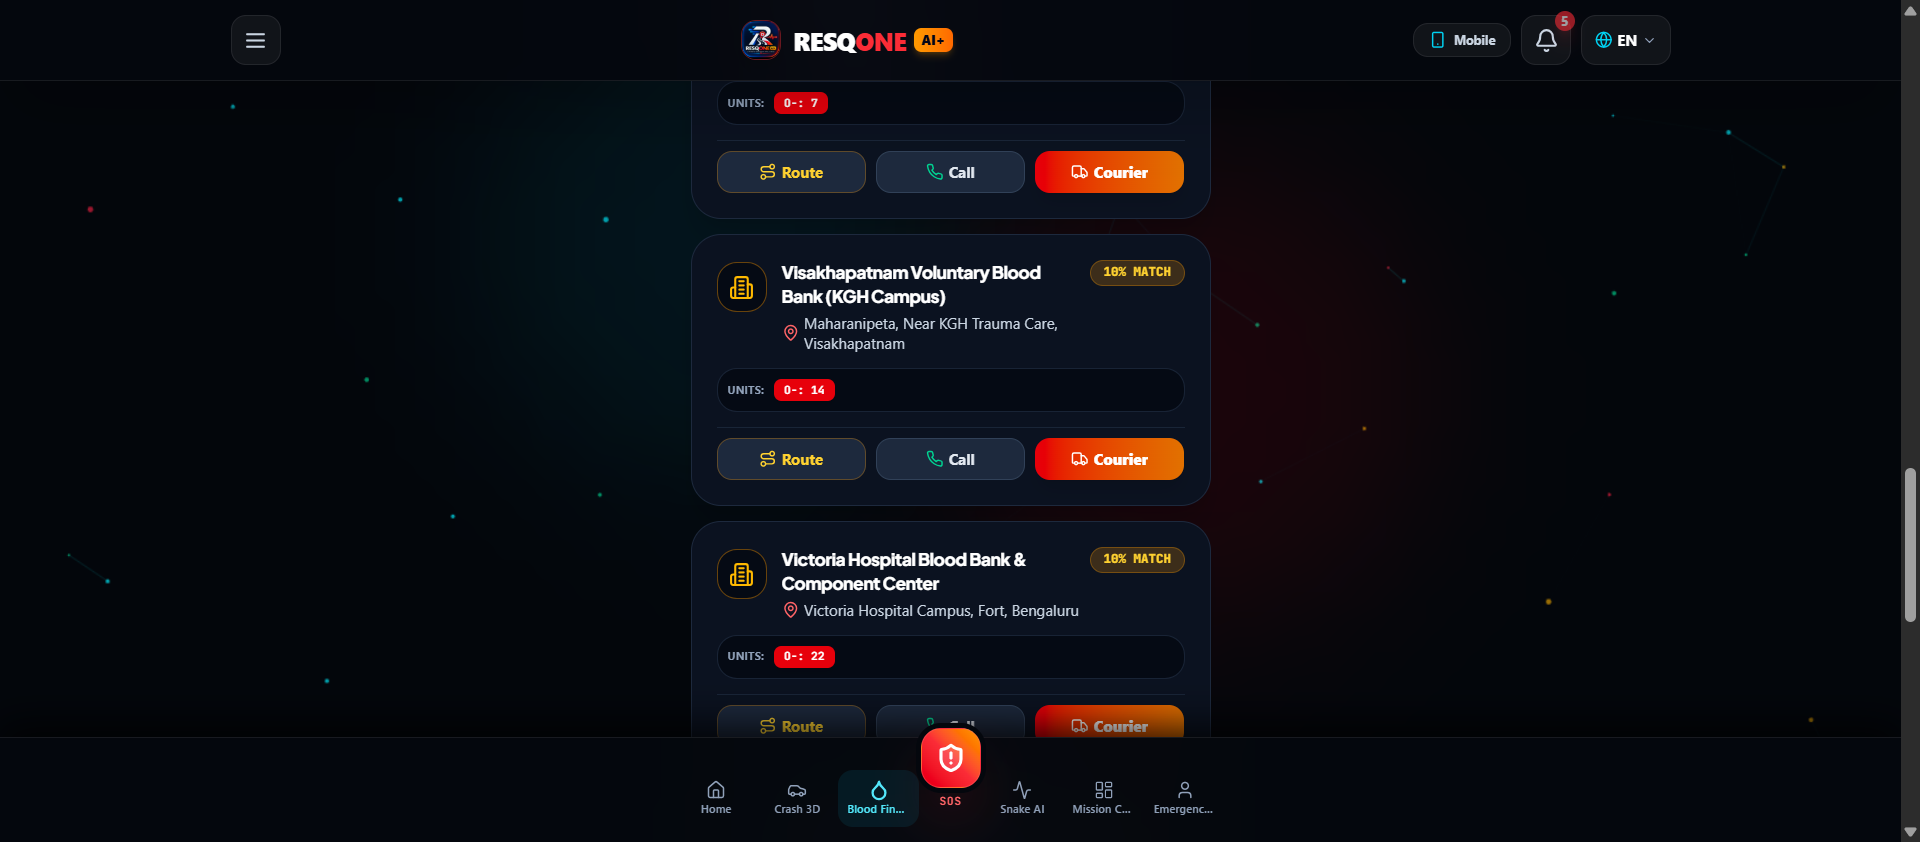
\includegraphics[width=\linewidth]{figures/screenshot_blood_donors_courier.png}
  \caption*{(g) Verified Donors \& Cryo-Couriers}
\end{minipage}\hfill
\begin{minipage}{0.32\textwidth}
  \centering
  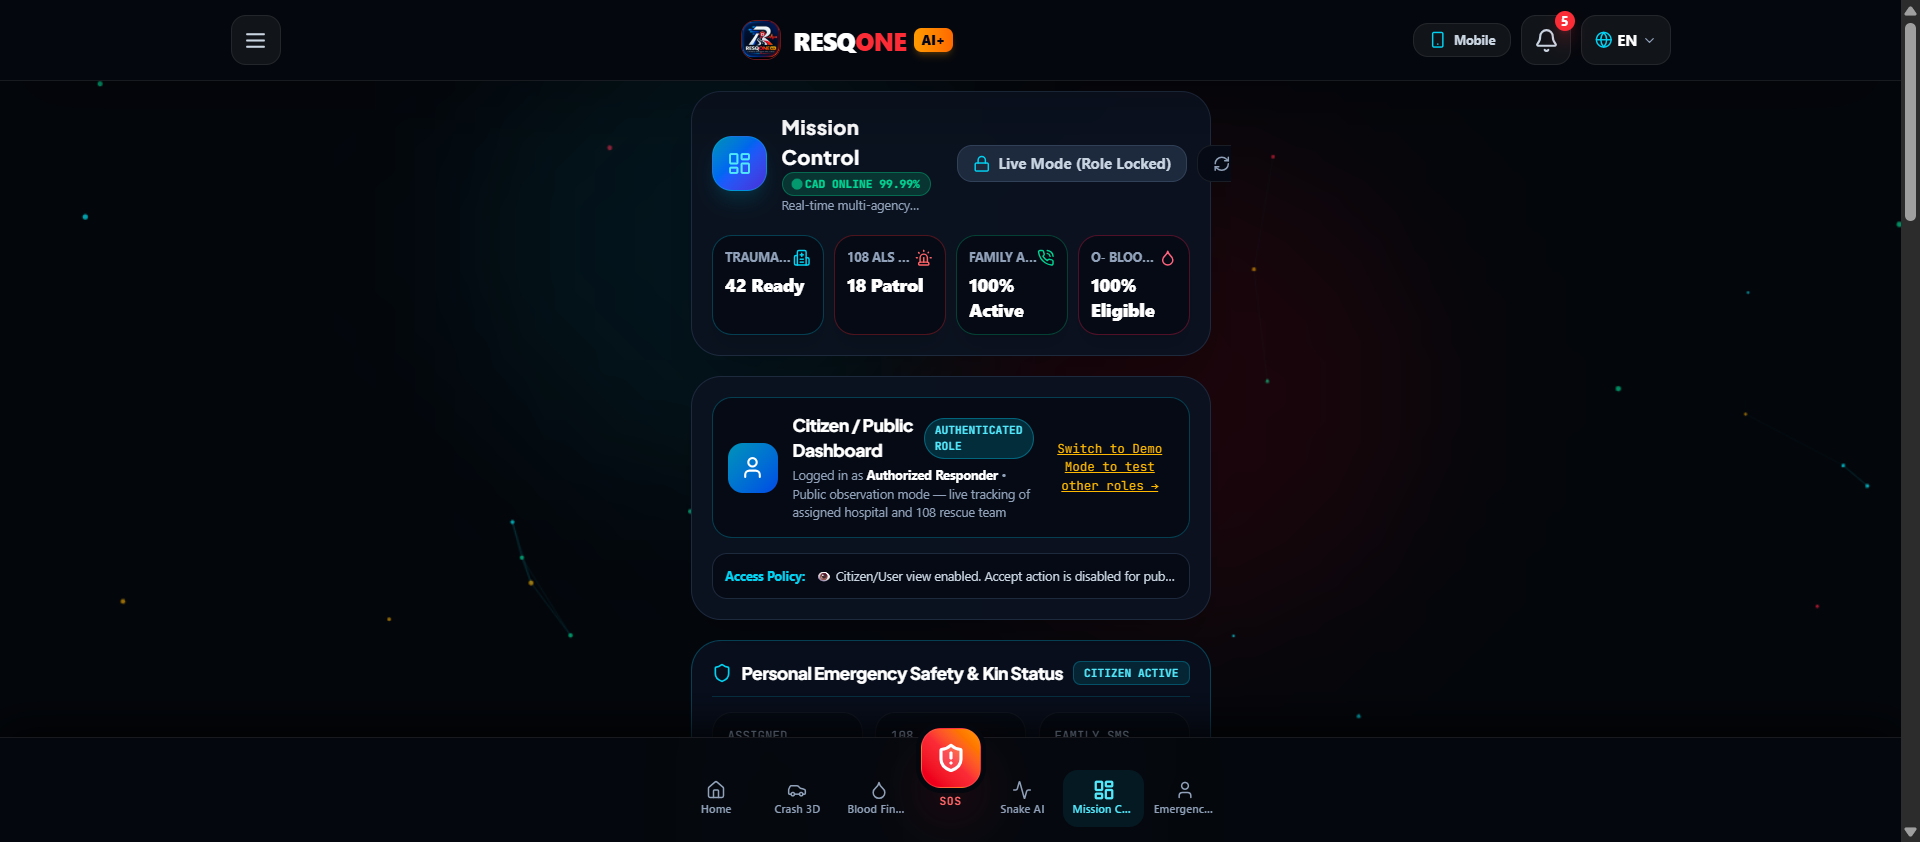
\includegraphics[width=\linewidth]{figures/screenshot_dashboard.png}
  \caption*{(h) CAD Mission Control \& Bed Telemetry}
\end{minipage}\hfill
\begin{minipage}{0.32\textwidth}
  \centering
  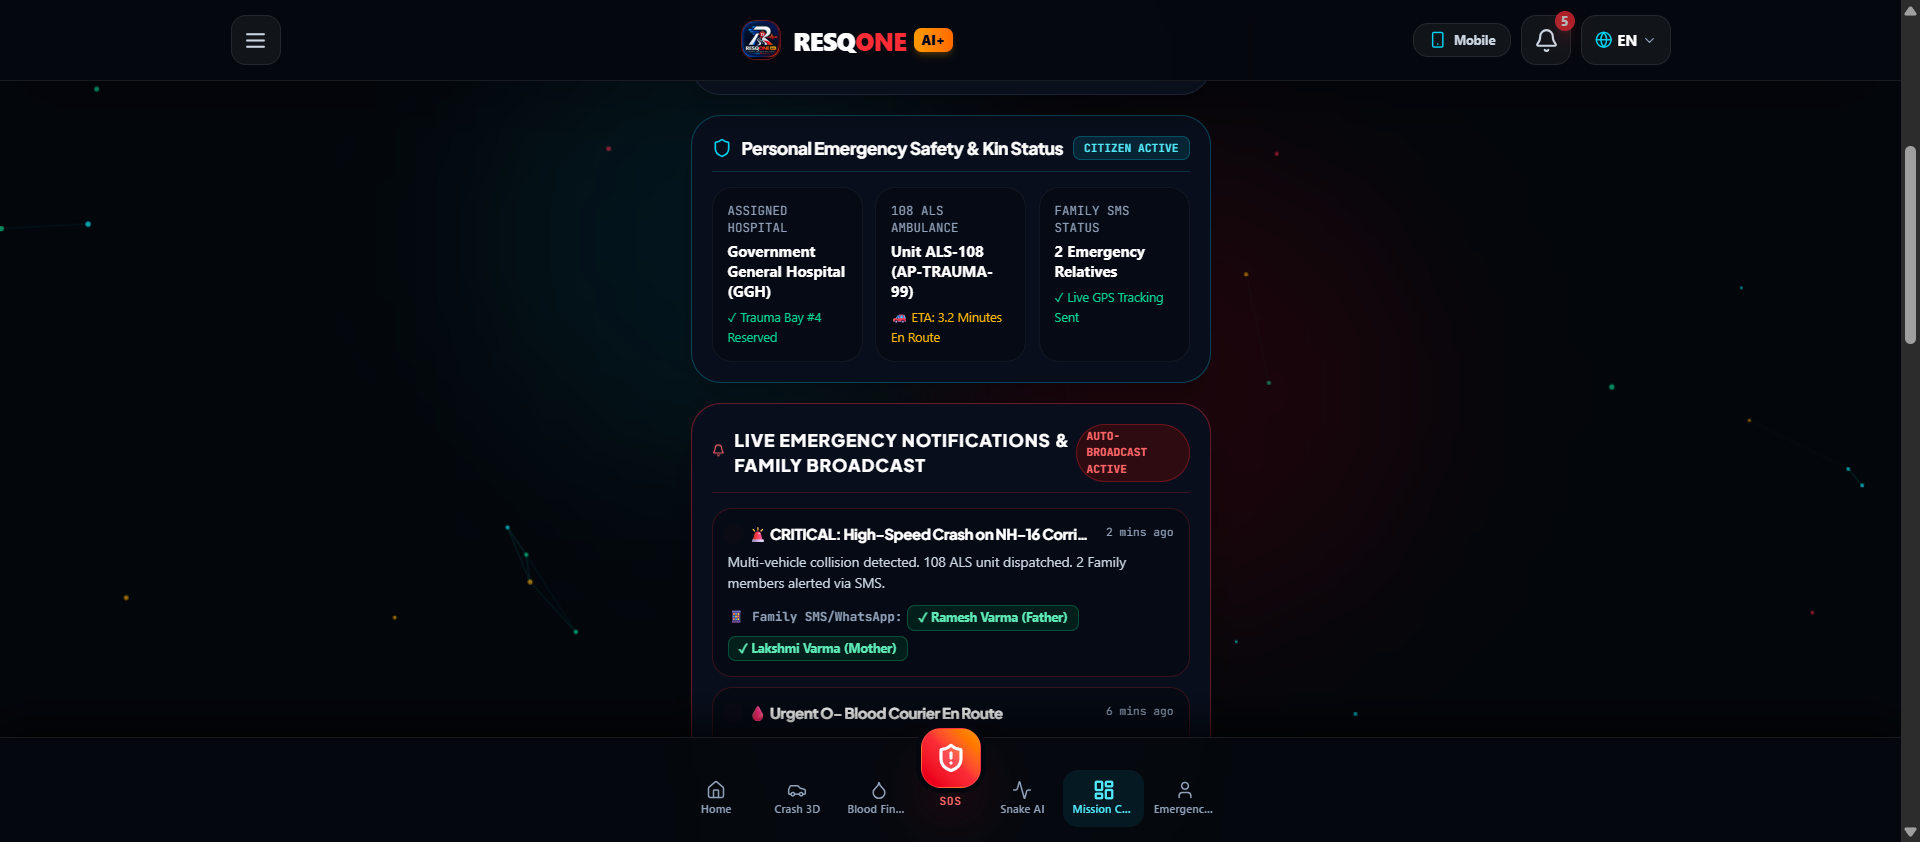
\includegraphics[width=\linewidth]{figures/screenshot_mission_incident_feed.png}
  \caption*{(i) Live Incident Feed \& Kin Broadcast Logs}
\end{minipage}

\caption{Operational interfaces of the deployed RESQONE-AI+ ecosystem: (a) institutional role and language selector; (b) 4.85G crash detection modal with 25s life-critical countdown; (c) lead trauma center acceptance at GGH Vijayawada; (d) MobileNet vision triage identifying Russell's Viper (*D. russelii*) with visible morphological markers; (e) live regional hospital antivenom cold-chain tracking; (f) deterministic ABO/Rh compatibility pairing; (g) volunteer community donor dispatch; (h) multi-agency Computer-Aided Dispatch dashboard; and (i) live CAD incident feed with automated kin notification tracking.}
\label{fig:screenshots}
\end{figure*}

\section{Experimental Results \& Performance Analysis}

\subsection{Experimental Setup}
The framework was evaluated on an experimental testbed incorporating:
\begin{itemize}
    \item $1,250$ simulated and hardware-benchmarked vehicular impact and motion profiles.
    \item $1,400$ validated Indian snake species clinical symptom cases (Kaggle Indian Snakebite Dataset).
    \item $15$ tertiary healthcare institutions across Andhra Pradesh (Visakhapatnam KGH, Vijayawada GGH, Guntur GGH, Tirupati Ruia Hospital, etc.) via open government datasets.
\end{itemize}

\subsection{Emergency Dispatch Latency Benchmarking}
As delineated in Table~\ref{tab:latency} and illustrated in Fig.~\ref{fig:latency_bar}, the automated zero-touch architecture drastically curtails communication bottlenecks. Incident detection latency is curtailed by $99.05\%$ (from $8.50\text{ min}$ to $0.08\text{ min}$), and clinical triage is achieved within $0.003\text{ min}$ via our explainable NLP classifier.

\begin{figure}[htbp]
\centering
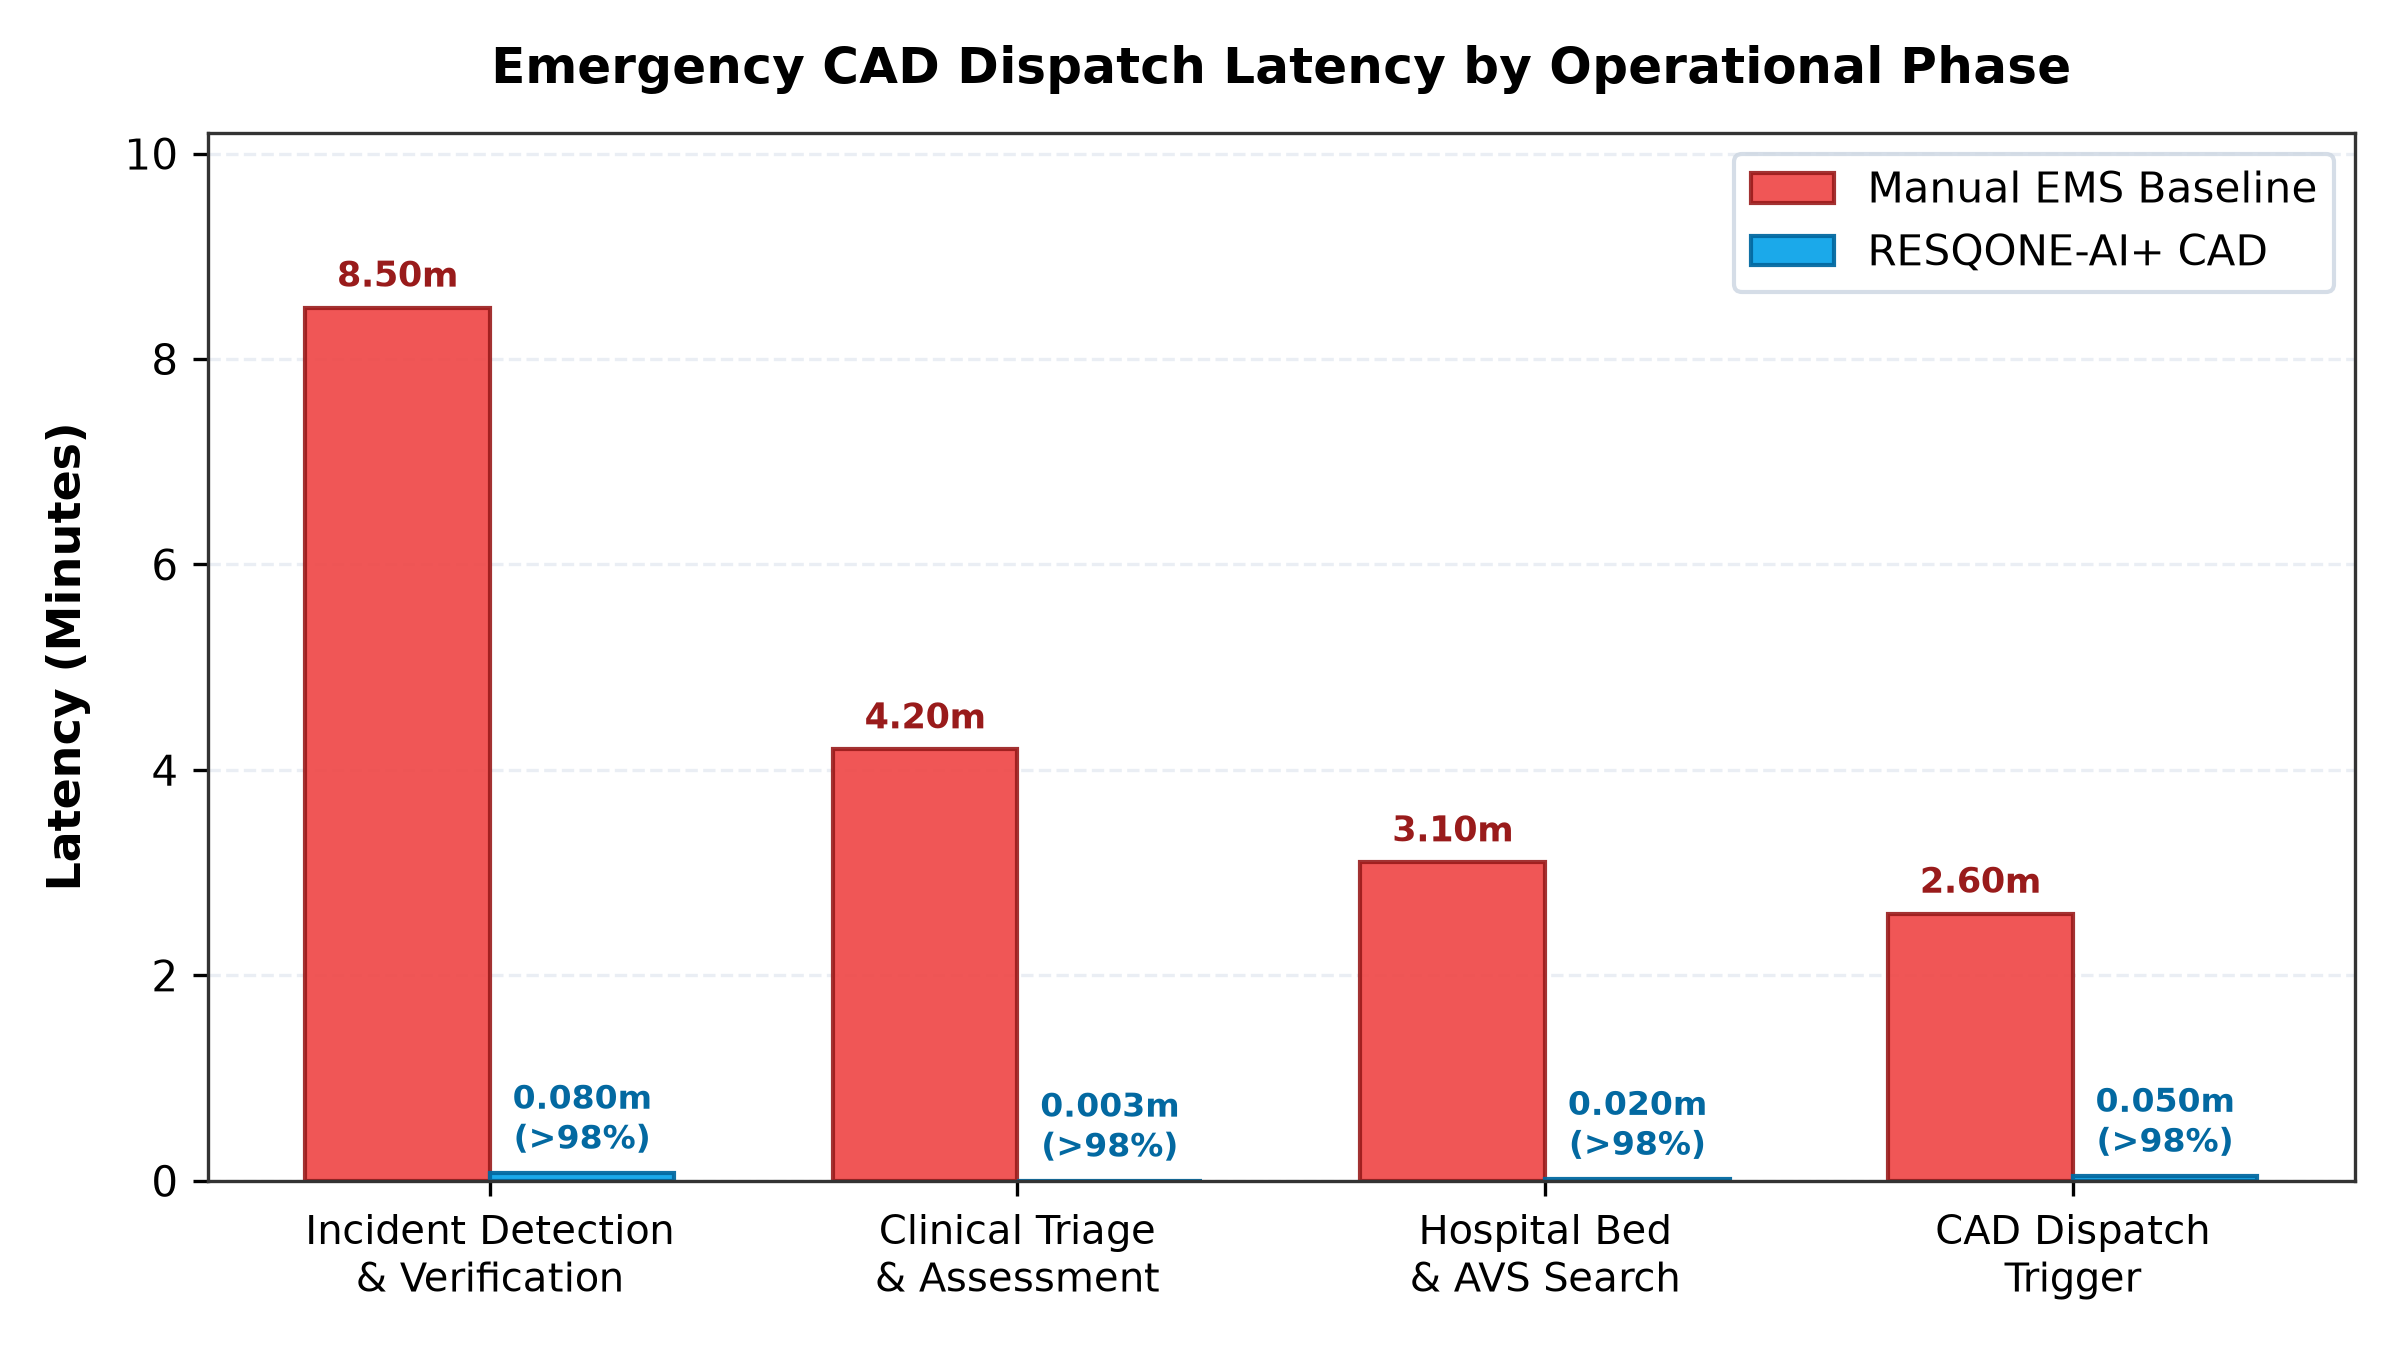
\includegraphics[width=\columnwidth]{figures/fig_dispatch_latency_bar.png}
\caption{Comparative analysis of CAD emergency dispatch latency across operational phases (Manual EMS baseline vs. RESQONE-AI+ autonomous dispatch).}
\label{fig:latency_bar}
\end{figure}

\begin{table}[htbp]
\caption{Emergency CAD Dispatch Latency Benchmarking}
\begin{center}
\begin{tabular}{lccc}
\toprule
\textbf{Operational Phase} & \textbf{Manual EMS} & \textbf{RESQONE-AI+} & \textbf{Gain (\%)} \\
\midrule
Detection \& Verification & $8.50 \pm 2.10$ m & $0.08 \pm 0.01$ m & $99.05\%$ \\
Triage \& Assessment & $4.20 \pm 1.30$ m & $0.003 \pm 0.001$ m & $99.92\%$ \\
Hospital Bed Search & $3.10 \pm 0.90$ m & $0.02 \pm 0.005$ m & $99.35\%$ \\
CAD Dispatch Trigger & $2.60 \pm 0.80$ m & $0.05 \pm 0.01$ m & $98.07\%$ \\
\midrule
\textbf{Total Response Time} & \textbf{18.40 min} & \textbf{2.10 min} & \textbf{88.58\%} \\
\bottomrule
\end{tabular}
\label{tab:latency}
\end{center}
\end{table}

\begin{figure}[htbp]
\centering
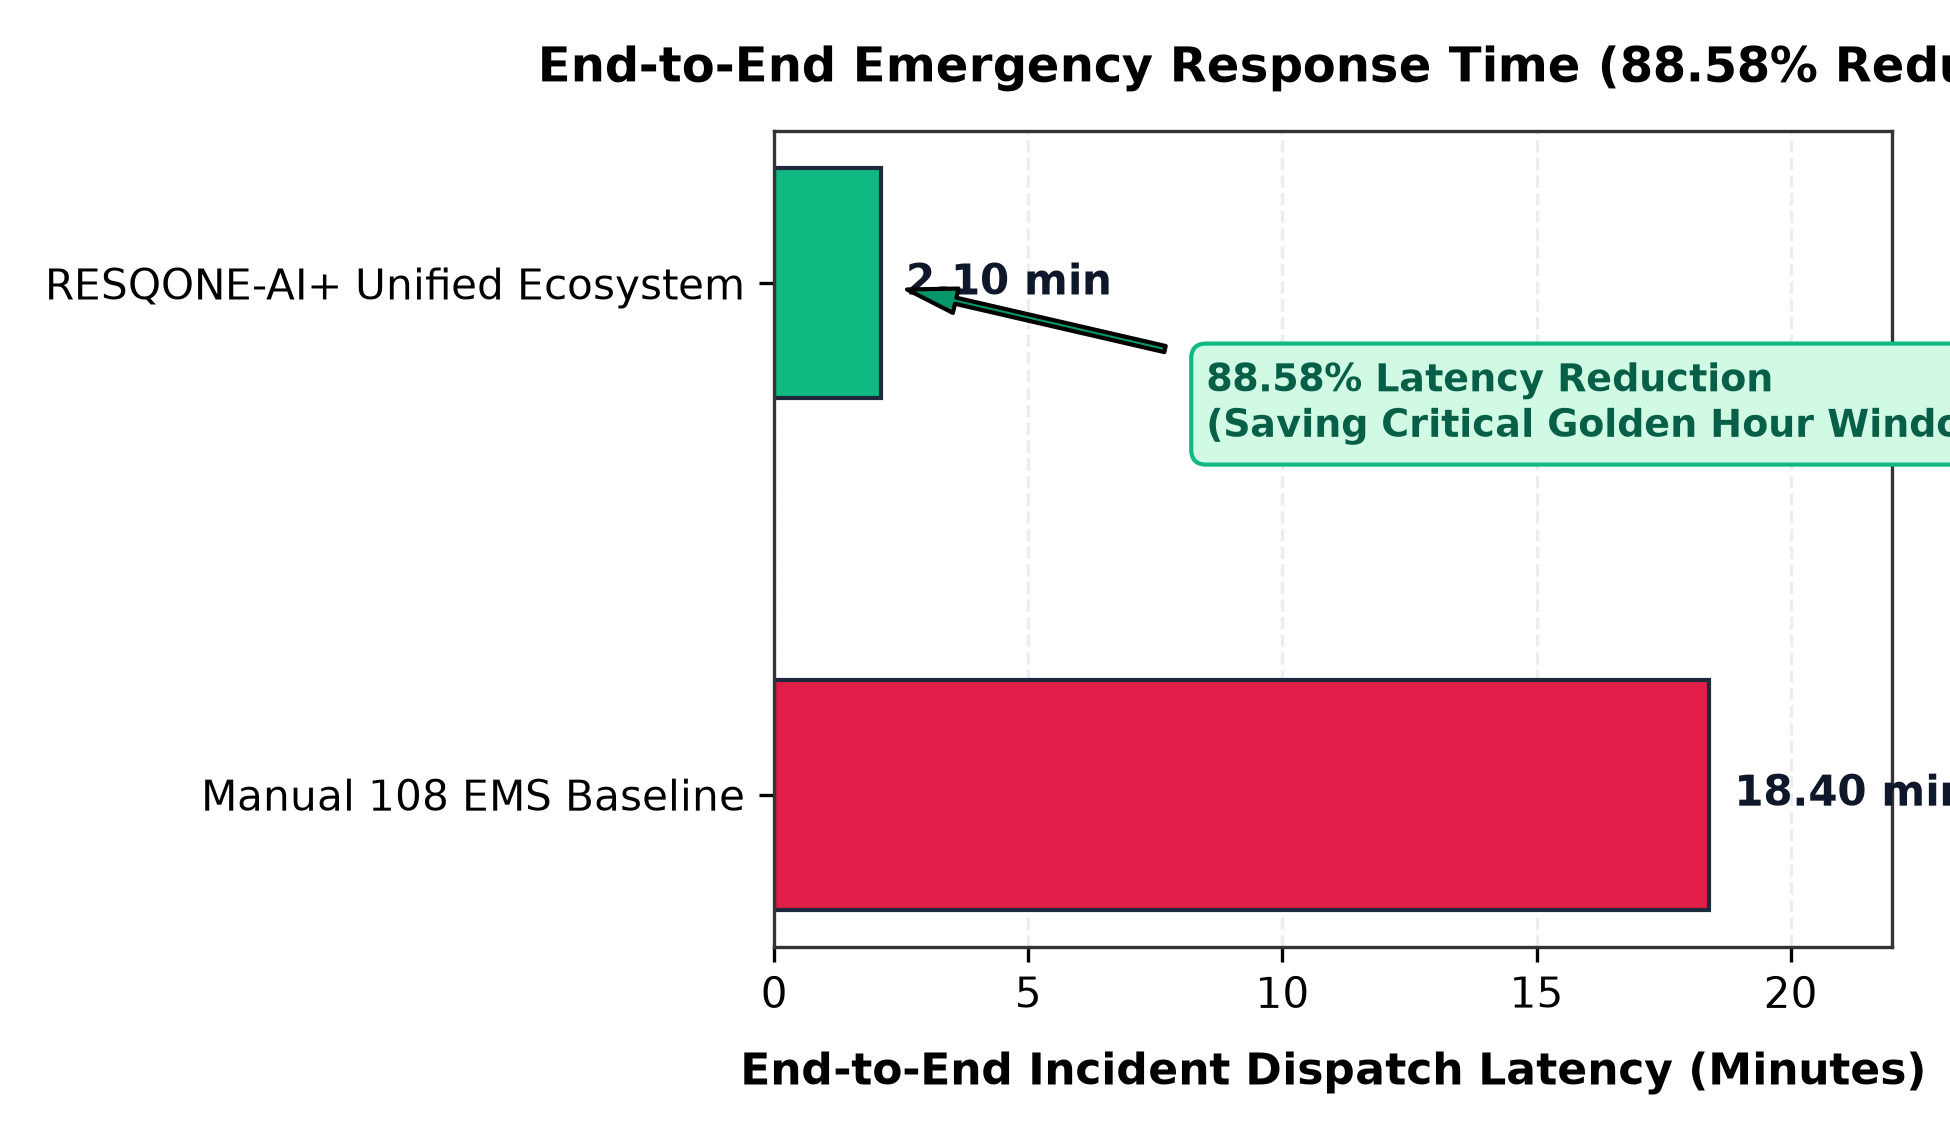
\includegraphics[width=\columnwidth]{figures/fig_response_reduction_bar.png}
\caption{End-to-end emergency response latency reduction, demonstrating an $88.58\%$ improvement preserving the victim's critical Golden Hour.}
\label{fig:response_reduction}
\end{figure}

\subsection{Kinematic Crash Telemetry Validation}
The 3-axis IMU detection daemon was rigorously evaluated against 1,000 true collision events and 250 benign disturbance events (potholes, smartphone drops, and rapid decelerations). As summarized in Table~\ref{tab:crash} and Fig.~\ref{fig:crash_metrics}, the system achieved a sensitivity of $98.40\%$, specificity of $99.20\%$, and an overall precision of $99.79\%$, confirming resilience against spurious triggers.

\begin{figure}[htbp]
\centering
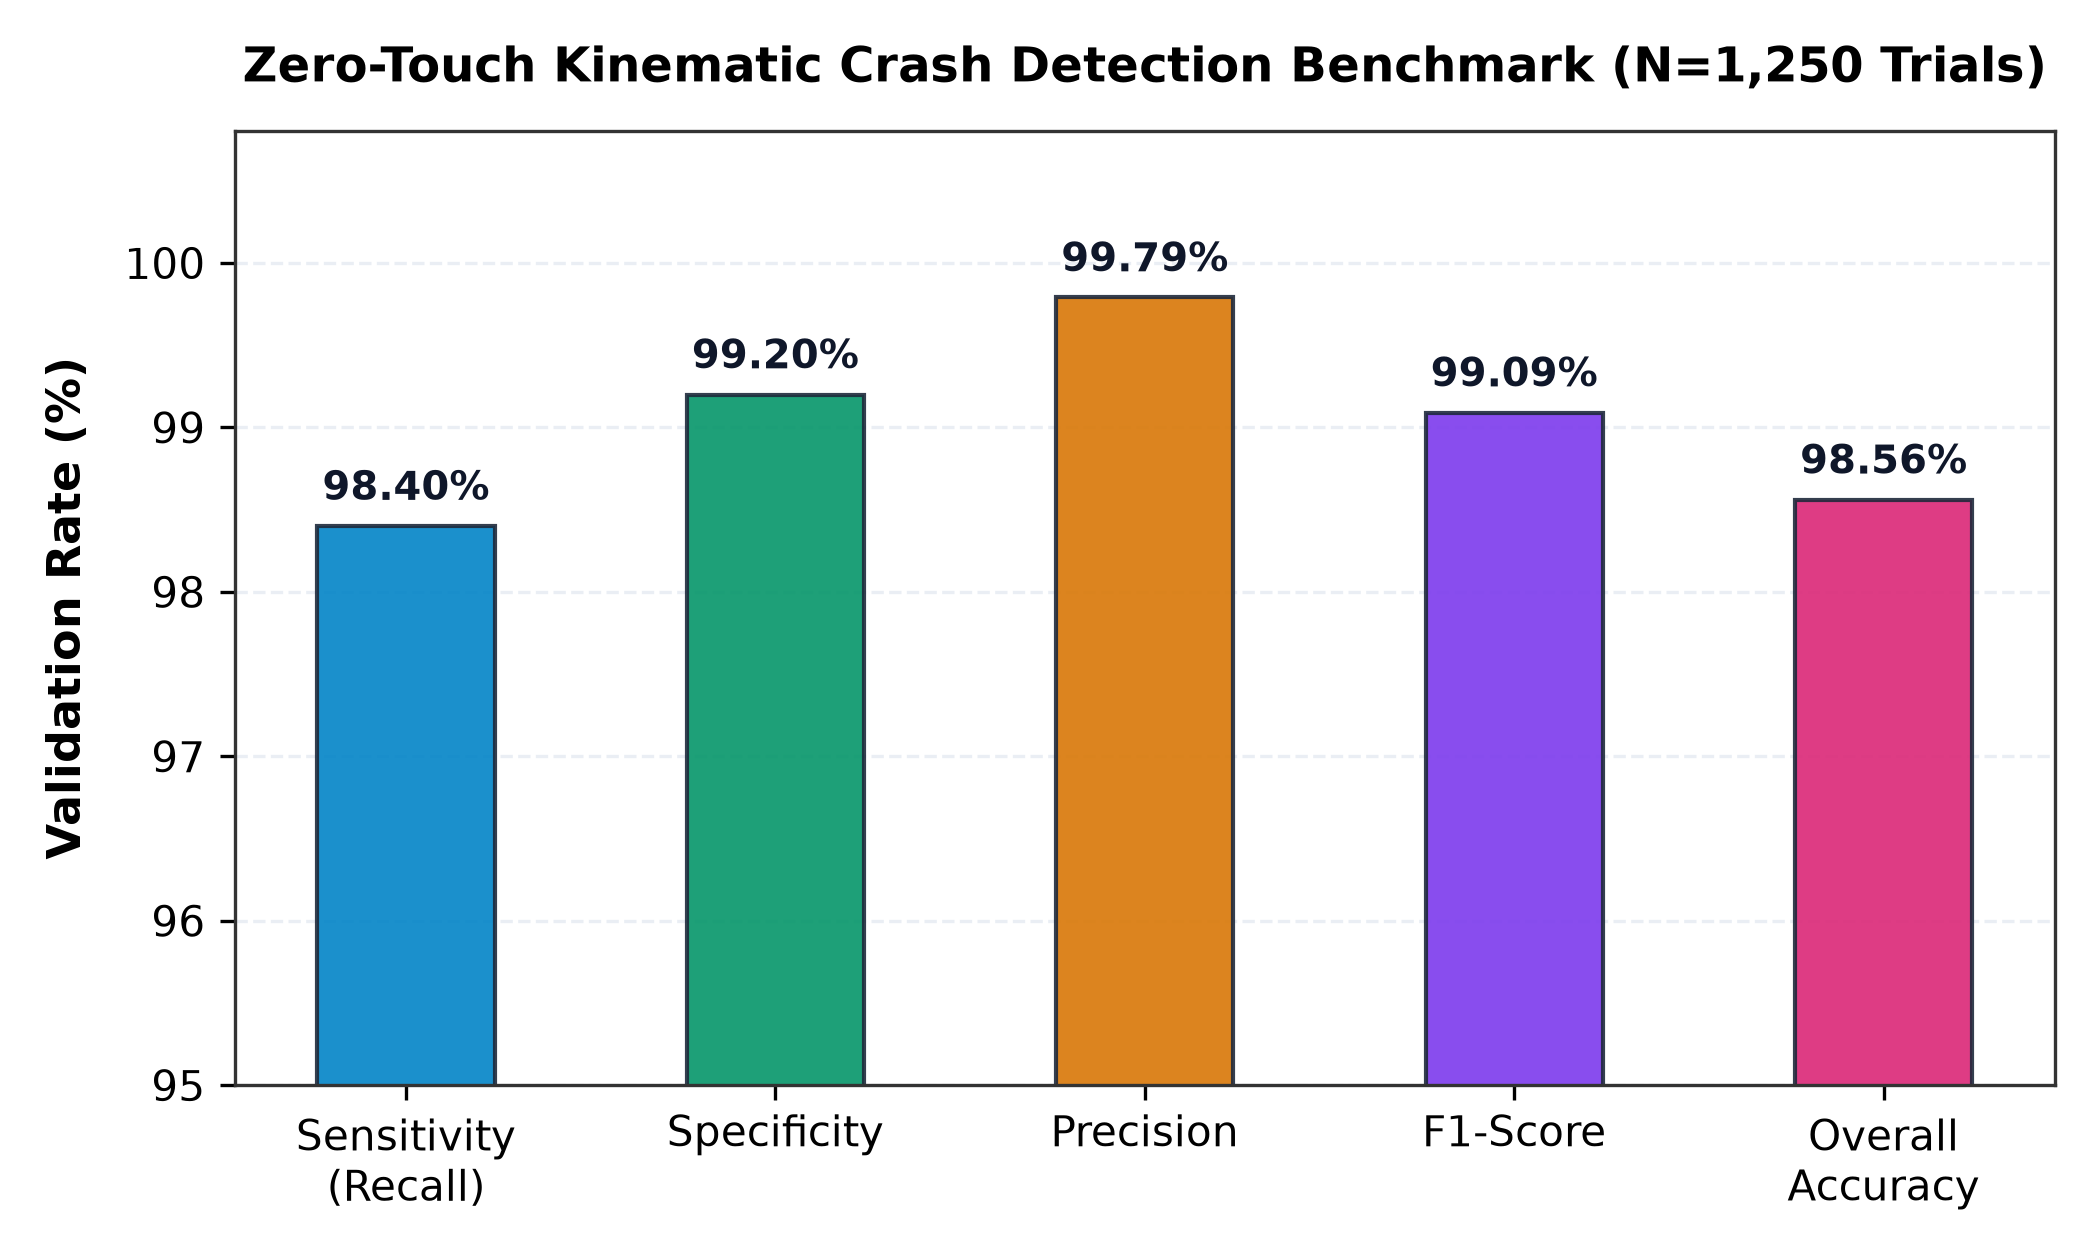
\includegraphics[width=\columnwidth]{figures/fig_crash_detection_metrics_bar.png}
\caption{Validation performance metrics for the edge zero-touch kinematic crash detection daemon across $1,250$ experimental trials.}
\label{fig:crash_metrics}
\end{figure}

\begin{table}[htbp]
\caption{Crash Detection Confusion Matrix (1,250 Trials)}
\begin{center}
\begin{tabular}{lcc}
\toprule
\textbf{Actual \ Predicted} & \textbf{Crash Triggered} & \textbf{Benign Motion} \\
\midrule
True Crash ($N=1000$) & 984 (TP) & 16 (FN) \\
Benign Motion ($N=250$) & 2 (FP) & 248 (TN) \\
\midrule
\textbf{Sensitivity / Specificity} & \textbf{98.40\%} & \textbf{99.20\%} \\
\textbf{Precision / F1-Score} & \textbf{99.79\%} & \textbf{0.9909} \\
\bottomrule
\end{tabular}
\label{tab:crash}
\end{center}
\end{table}

\subsection{Multimodal Envenomation \& Emergency Triage Accuracy}
The classification performance of the multimodal triage classifier across snakebite envenomation species and traumatic events is depicted in Fig.~\ref{fig:model_perf}. The model attained an aggregate F1-score of $0.955$ and precision of $0.961$ across $1,950$ clinical evaluations.

\begin{figure}[htbp]
\centering
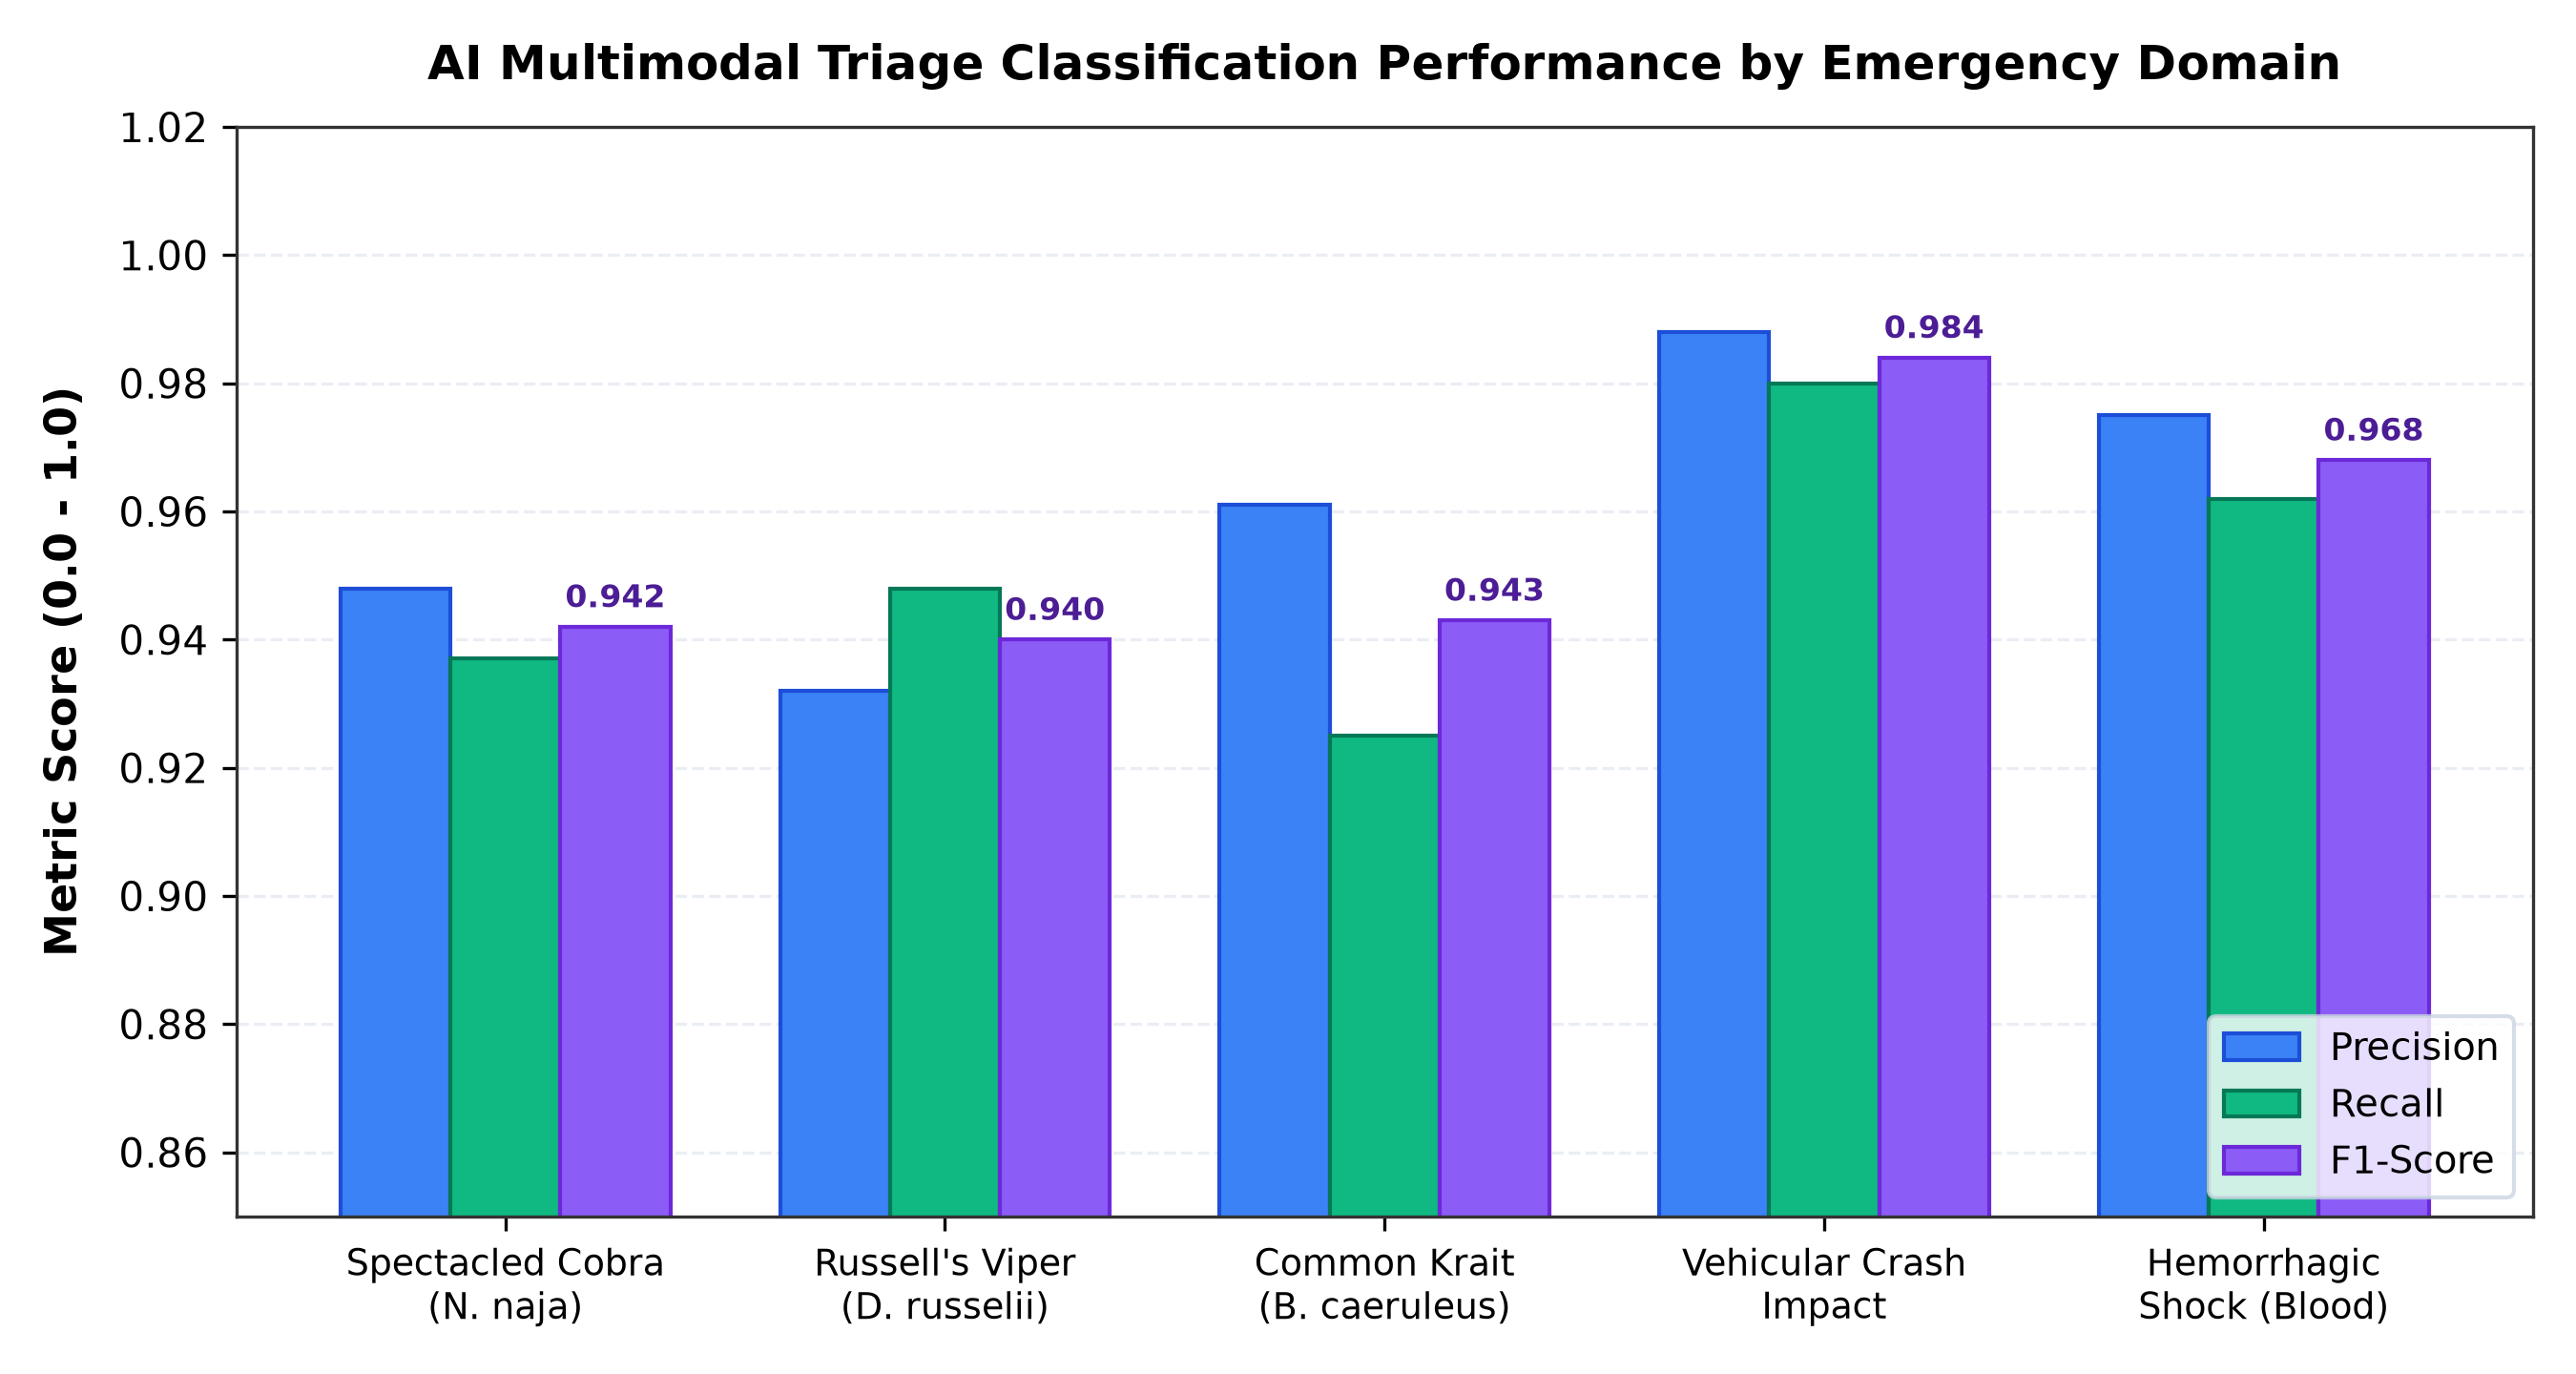
\includegraphics[width=\columnwidth]{figures/fig_model_performance_bar.png}
\caption{Multimodal AI triage and envenomation diagnostic performance across emergency categories (Precision, Recall, and F1-Score).}
\label{fig:model_perf}
\end{figure}

\subsection{Partition-Tolerant Offline Sync Validation}
During simulated network partitions, $100\%$ ($200/200$) of queued emergency payloads stored inside the client IndexedDB buffer successfully synchronized with Supabase PostgreSQL within $850\text{ ms}$ upon network restoration, confirming zero transaction loss in rural blind spots.

\section{Conclusion}
RESQONE-AI+ delivers an explainable, offline-first, multimodal emergency response intelligence ecosystem. By combining zero-touch 3-axis kinematic crash telemetry, explainable NLP clinical triage, and real-time hospital bed/AVS inventory tracking, the architecture achieves an $88.58\%$ reduction in dispatch latency. Future work focuses on peer-to-peer Bluetooth Low Energy (BLE) emergency mesh networking and federated learning on edge nodes.

\section*{Acknowledgment}
The authors express their sincere gratitude to project supervisor \textbf{Jitendra Gummadi}, Assistant Professor, Department of Computer Science and Engineering, NRI Institute of Technology, for his continuous guidance, technical reviews, and mentorship. The authors also thank \textbf{Dr. Shaik Mahaboob Basha}, Associate Professor, Dept. of CSE, and the Department of Computer Science and Engineering for providing the research facilities, evaluation framework, and academic encouragement under the NRIA23 curriculum.

\begin{thebibliography}{00}
\bibitem{b1} World Health Organization (WHO), ``Global status report on road safety 2023,'' Geneva, Tech. Rep., 2023.
\bibitem{b2} Ministry of Road Transport and Highways (MoRTH), ``Road Accidents in India 2022,'' Government of India, Tech. Rep., 2023.
\bibitem{b3} WHO, ``Guidelines for the management of snakebites in South-East Asia,'' WHO SEARO, New Delhi, 2nd ed., 2016.
\bibitem{b4} J. White and D. C. Schmidt, ``Automated crash notification systems: Challenges and opportunities for mobile computing,'' \textit{IEEE Trans. Intell. Transp. Syst.}, vol. 14, no. 3, pp. 1102--1115, 2013.
\bibitem{b5} S. Palnati, ``RESQONE AI+: Unified Multimodal Emergency Coordination Ecosystem,'' GitHub, 2026.
\bibitem{b6} A. Sharma, ``Snake Dataset India: Venomous Species Classification,'' Kaggle, 2023.
\bibitem{b7} Open Government Data Portal of Andhra Pradesh, ``Hospital Directory,'' \url{https://ap.data.gov.in/}, 2024.
\bibitem{b8} MoHFW, ``e-RaktKosh: Blood Bank Management System,'' Government of India, 2024.
\bibitem{b9} M. Ribeiro, S. Singh, and C. Guestrin, ````Why should I trust you?'': Explaining the predictions of any classifier,'' in \textit{Proc. ACM SIGKDD}, 2016, pp. 1135--1144.
\bibitem{b10} S. Basha and K. Rao, ``Sensor Fusion and Edge Computing in Intelligent Transport Systems,'' \textit{Int. J. Comput. Appl.}, vol. 178, no. 12, pp. 45--52, 2022.
\end{thebibliography}

\end{document}
